\documentclass[twocolumn,floatfix,aps,prd,nofootinbib]{revtex4-2}

\usepackage[T1]{fontenc}
\usepackage{graphicx}
\usepackage{amssymb}
\usepackage{amsmath}
\usepackage{xcolor}
\usepackage{hyperref}
\usepackage{placeins}
\usepackage[protrusion=true,expansion=false]{microtype}
\usepackage{tikz}
\usepackage{pgfplots}
\usetikzlibrary{arrows.meta,positioning,plotmarks,fit,calc}
\usepgfplotslibrary{groupplots}
\pgfplotsset{compat=1.18}
\graphicspath{{../figures/}}

\hypersetup{
    colorlinks=true,
    linkcolor=blue,
    filecolor=magenta,
    urlcolor=blue,
    citecolor=blue,
}
\urlstyle{same}
\emergencystretch=2em

\begin{document}

\title{Matter-first automated discovery of transient spacetime shortcuts}

\author{Nikita M. Shirokov}
\email{shirokov.nm@phystech.edu}
\affiliation{Independent Researcher, Moscow, Russia}
\date{\today}

\begin{abstract}
We present an automated matter-first pipeline for discovering warp
precursors---transient spacetime shortcuts. An optimizer proposes scalar
matter, \texttt{GRTresna} solves the constraints, \texttt{GRTeclyn} evolves the
full $3{+}1$ Einstein equations, and null geodesics integrated through the
\emph{time-evolving} metric test whether light arrives earlier than in flat
space. Quality-diversity search over a 39-dimensional bicomplex Q-ball genome
yields a five-lump champion (candidate~146) with two canonical and three
phantom (negative-energy) sources. Freely falling observers receive the photon
$7.6\%$ early by their own clocks---the physical magnitude of the shortcut,
against $20.2\%$ between fixed coordinate endpoints---stable across resolution
and domain ladders and reproduced with the ignition controller off.
Field-by-field ablation attributes the transport to conformal spatial
contraction and lapse elevation, not to frame dragging: deleting the shift
entirely \emph{increases} the shortcut. A companion pure-geometry atlas
explains why. Its kinematic ceiling is $48.5\%$ for shift-dominated
(Alcubierre) topologies but only $21.8\%$ for the curvature-dominated branch
the champion sources and nearly saturates---a Pareto frontier between kinematic
strength and dynamical sourceability. A matched canonical-only search finds no
advantage at all. The channel is transient: the matter disperses and the
residue collapses to an apparent horizon by $t\approx27$.
\end{abstract}

\maketitle

\section{Introduction}
\label{sec:intro}

The goal of this work is an \emph{automatic discovery pipeline} for
faster-than-light (FTL) warp precursors, in the spirit of recent automated
theory- and pipeline-discovery efforts in fundamental
physics~\cite{alexander2026albert,qiu2026collideragent}. We define a warp
precursor---a transient \emph{spacetime shortcut}---as a
constraint-satisfying matter configuration that generates an effective null
timing advantage prior to its own dispersal: null rays between prescribed fixed
endpoints in the weak-field region traverse the curved spacetime in less
coordinate time than the matched flat-space path---never local superluminal
motion outside the light cone. ``FTL'' and ``null shortcut'' are used
interchangeably for that operational claim throughout. Rather
than hand-crafting a metric and hoping the implied stress-energy is physical,
we want a closed loop that proposes candidates, evolves them under the
Einstein equations, and retains only those that pass a gauge-invariant
transport test.

The standard route is \emph{geometry-first} (equivalently metric-first): one
prescribes $g_{\mu\nu}$, reads off $T_{\mu\nu}=G_{\mu\nu}/8\pi$, and studies
frozen slices~\cite{alcubierre94,natario02,helmerich2024warpfactory}.
That recipe is poorly conditioned for automated search. Most deformations of
$g_{\mu\nu}$ violate the constraints, have no local matter realization, or fail
as soon as time advances, so an archive of hundreds of such candidates fills
with numerical failures rather than competing mechanisms.

We therefore invert the loop (Fig.~\ref{fig:matter_first}): the optimizer
proposes matter, \texttt{GRTresna} builds the constraint-satisfying initial
slice, \texttt{GRTeclyn}~\cite{grteclyn,grchombo} advances the spacetime, and
probes ask whether a null shortcut appears (the two codes are detailed in
Sec.~\ref{sec:tools}). The fractional advantage is $f_{\rm geo}$
[Eq.~\eqref{eq:f_geo}], quoted throughout as a percentage: $f_{\rm geo}=20\%$
means the curved transit is one fifth shorter than the flat comparison. By classical theorems on
superluminal travel and gravitational time
delay~\cite{olum98,gaowald00,visser00}, any such advantage between endpoints
in the (near-)flat region requires violation of the null energy condition,
and generic warp-drive spacetimes share this
requirement~\cite{santiago2022}; the phantom sector introduced below is the
controlled realization of that necessity in our matter model.

\begin{figure*}[tbp]
\centering
\resizebox{0.94\textwidth}{!}{%
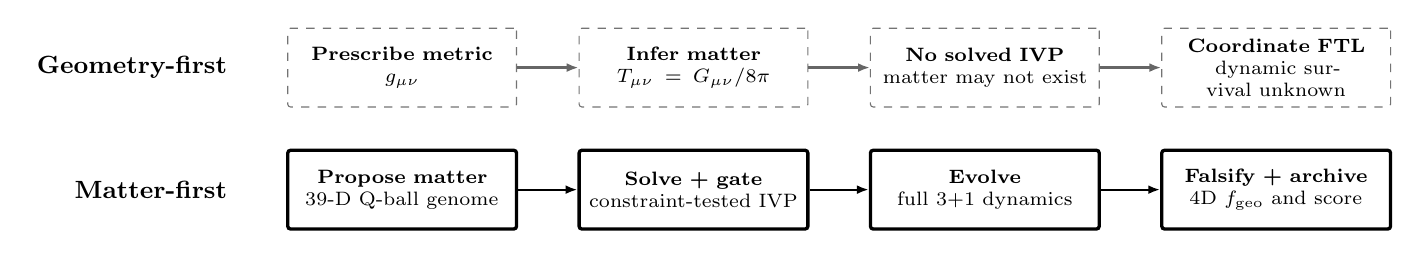
\begin{tikzpicture}[
  font=\scriptsize,
  stagebox/.style={draw, rounded corners=1pt, align=center,
               text width=28mm, minimum height=10mm, inner sep=1.5pt},
  classic/.style={stagebox, draw=black!55, dashed},
  ours/.style={stagebox, very thick},
  flow/.style={-{Latex[length=1.5mm]}, thick},
  row/.style={font=\bfseries\small, anchor=east}
]
\node[row] at (0,0) {Geometry-first};
\node[classic] (g1) at (2.1,0) {\textbf{Prescribe metric}\\$g_{\mu\nu}$};
\node[classic] (g2) at (5.8,0) {\textbf{Infer matter}\\$T_{\mu\nu}=G_{\mu\nu}/8\pi$};
\node[classic] (g3) at (9.5,0) {\textbf{No solved IVP}\\matter may not exist};
\node[classic] (g4) at (13.2,0) {\textbf{Coordinate FTL}\\dynamic survival unknown};
\draw[flow, draw=black!60] (g1)--(g2);
\draw[flow, draw=black!60] (g2)--(g3);
\draw[flow, draw=black!60] (g3)--(g4);

\node[row] at (0,-1.55) {Matter-first};
\node[ours] (m1) at (2.1,-1.55) {\textbf{Propose matter}\\39-D Q-ball genome};
\node[ours] (m2) at (5.8,-1.55) {\textbf{Solve + gate}\\constraint-tested IVP};
\node[ours] (m3) at (9.5,-1.55) {\textbf{Evolve}\\full $3{+}1$ dynamics};
\node[ours] (m4) at (13.2,-1.55) {\textbf{Falsify + archive}\\4D $f_{\rm geo}$ and score};
\draw[flow] (m1)--(m2);
\draw[flow] (m2)--(m3);
\draw[flow] (m3)--(m4);
\end{tikzpicture}}
\caption{Geometry-first versus matter-first discovery. Dashed: prescribe a
metric and infer its stress-energy. Solid: propose matter, solve and test an
initial-value problem (IVP), evolve it, and archive only candidates that pass
the 4D null-transport test.}
\label{fig:matter_first}
\end{figure*}

This criterion is the acceptance test, not a post-hoc diagnostic. A warp
precursor is useful only if it changes what light can do between fixed distant
observers, and local coordinate signal speeds, lapse and shift artifacts, or a
positive frozen-slice diagnostic can all look ``superluminal'' while no ray
actually connects the endpoints sooner once the metric evolves.

Equally important is the \emph{scoring metric} that turns each evolution into
the fitness $S(\theta)$ [Eq.~\eqref{eq:score}], because MAP-Elites converges to
whatever $S$ rewards. Earlier campaigns with weaker objectives reliably
``cheated''---harvesting coordinate proxies while the matter dispersed, banking
frozen-slice positives that failed the evolving test, or climbing scores
through outright numerical pathologies. The gates that close those routes are
detailed in Sec.~\ref{sec:scoring}.

The search engine is MAP-Elites~\cite{mouret15}, a quality-diversity algorithm
that keeps one elite per cell of a behavior archive rather than a single global
optimum---preferred over a pure CMA-ES~\cite{hansen01} hill-climb, which
collapses onto one basin, and over reinforcement learning, which would need
dense credit assignment across expensive GPU evolutions with sparse rewards.
CMA-ES then warm-starts from the archive champion and refines it locally
(Sec.~\ref{sec:methodology}). Both discovery stages run on a deliberately
coarse grid chosen for throughput; production claims are deferred to the
high-quality (HQ) replay and resolution matrix (Sec.~\ref{sec:stages}).

The headline champion (candidate~146) relies on a phantom scalar sector, so it
does \emph{not} bypass the energy-condition violations required of FTL
spacetimes~\cite{olum98,gaowald00,santiago2022}. Its value is a demonstration
that an automated, matter-first Cauchy pipeline can discover, construct, and
dynamically track constraint-satisfying FTL geometries---a necessary first step
toward searching the positive-energy sector~\cite{lentz21,fell21} with the same
falsification stack. As a first probe, a matched canonical-only
(positive-energy) search within the present ansatz returns
$f_{\rm geo}^{\rm evol}=0$ for every accepted evaluation
(Sec.~\ref{sec:canonical_bound}).

\subsection{Contributions}
\label{subsec:contributions}

Three commitments separate this pipeline from geometry-first studies, and each
is a contribution of the paper.
\begin{enumerate}
    \item \textbf{A solved initial-value problem.} Every candidate begins as
    constraint-clean data from physical scalar sources, not a coordinate
    script, produced by an end-to-end loop---MAP-Elites proposal, CMA-ES local
    refinement, constraint solve, GPU evolution, matched scoring---with one
    explicit reward rule applied to every evaluation
    (Secs.~\ref{sec:pipeline}--\ref{sec:methodology}).
    \item \textbf{Dynamic feedback.} Full CCZ4 evolution, so dispersing matter
    collapses the channel and cannot be scored around; claims are promoted
    through a hierarchical protocol ending in a Richardson resolution ladder
    on the frozen champion (Sec.~\ref{sec:stages}).
    \item \textbf{4D geodesic falsification.} The headline diagnostic is
    \texttt{ftl\_geo\_evolving}---null rays integrated through the
    \emph{time-evolving} metric stack. Frozen-slice geodesics are retained as
    diagnostics but never as the transport certificate. The surviving
    candidate's limits are reported as explicitly as its successes: dispersing
    exotic matter, a transient ignition controller, and a late-time collapse to
    an apparent horizon once the exotic support is gone---not passenger
    transport (Sec.~\ref{sec:discussion}).
\end{enumerate}

\section{Matter-First Pipeline}
\label{sec:pipeline}

\subsection{Two-code toolchain}
\label{sec:tools}

Two open numerical-relativity codes carry the loop.
\texttt{GRTresna}~\cite{grtresna} is a constraint solver: given a matter
configuration it returns constraint-satisfying initial data
$(\gamma_{ij},K_{ij},\phi,\Pi)$ on the initial slice, so that the Hamiltonian
and momentum constraints hold before any evolution.
\texttt{GRTeclyn}~\cite{grteclyn,grchombo} is a GPU-accelerated,
AMReX-based~\cite{amrex} code that evolves those data forward with the CCZ4
formulation~\cite{alic12} of the Einstein equations under moving-puncture
gauge~\cite{campanelli06,baker06}. Neither code is told what metric to
produce; the geometry is whatever the proposed matter sources. One evaluation
therefore maps a parameter vector $\theta$ to a scalar fitness---$\theta
\rightarrow$ initial data $\rightarrow$ \texttt{GRTeclyn} $\rightarrow$
diagnostics $\rightarrow S(\theta)$---with post-processing probes reducing the
evolution to the fitness that steers the next proposal
(Fig.~\ref{fig:pipeline}).

\subsection{Matter model: canonical and phantom scalar sectors}
\label{sec:phantom_action}

The matter is built from complex scalar fields with canonical Klein--Gordon
dynamics; the production model carries two independent fields, each with a
conjugate momentum $\Pi$ and the sextic potential $V$ of
Eq.~\eqref{eq:sextic}. In the $3{+}1$ split, a complex scalar contributes an
energy density $\rho$ and a momentum density $S_i$ that act as the sources in
the Hamiltonian and momentum constraints,
\begin{equation}
\rho=\tfrac12\psi^{-4}|\tilde\nabla\phi|^2+\tfrac12|\Pi|^2+V(\phi),
\qquad
S_i=-\mathrm{Re}\!\left(\Pi^{*}\partial_i\phi\right),
\label{eq:scalar_sources}
\end{equation}
where $\psi$ is the conformal factor and $\tilde\nabla$ the conformal spatial
gradient. The three terms in $\rho$ are the gradient (spatial shape), kinetic
(time variation), and potential (rest) energy of the field, while $S_i$ is
nonzero only when the field oscillates in time ($\Pi\neq0$) with a spatial
gradient. Equation~\eqref{eq:scalar_sources} is the precise statement of ``the
matter tells the geometry what to be'': $\theta$ sets $\phi$ and $\Pi$, and
\texttt{GRTresna} returns the $(\gamma_{ij},K_{ij})$ consistent with them.

Because the exotic sign is central to the claim, we state exactly what the
\texttt{grtresna\_bicomplex\_scalar} model integrates. Each complex scalar is
canonical, with action
\begin{equation}
S[\Phi]=\int d^4x\,\sqrt{-g}\left(
-g^{\mu\nu}\partial_\mu\Phi^{*}\partial_\nu\Phi-V(|\Phi|)\right),
\label{eq:canonical_action}
\end{equation}
Writing $\Pi=n^\mu\partial_\mu\Phi$ for the conjugate momentum along the
normal $n^\mu$, both the canonical field $\Phi_{+}$ and the exotic field
$\Phi_{-}$ obey the \emph{same} $3{+}1$ Klein--Gordon system,
\begin{align}
\partial_t\Phi_{\pm} &= \alpha\,\Pi_{\pm}+\beta^i\partial_i\Phi_{\pm},
\nonumber\\
\partial_t\Pi_{\pm} &= \beta^i\partial_i\Pi_{\pm}
   +\alpha\!\left(K\,\Pi_{\pm}+\gamma^{ij}D_iD_j\Phi_{\pm}
   -\frac{\partial V}{\partial\Phi_{\pm}^{*}}\right)\nonumber\\
&\quad +\gamma^{ij}\partial_i\alpha\,\partial_j\Phi_{\pm},
\label{eq:kg_evolution}
\end{align}
with $D_i$ the spatial covariant derivative and $\alpha,\beta^i,\gamma_{ij}$
the usual lapse, shift, and spatial metric. Both sectors are therefore governed
by identical right-sign (non-ghost) kinetic operators, free of the gradient and
ghost instabilities that afflict a genuine phantom Lagrangian
$\mathcal L=+\partial_\mu\phi\,\partial^\mu\phi^{*}-V$.

The exotic character enters at exactly one place: the \emph{gravitational
coupling}. The two sectors add to the Einstein source with opposite sign,
\begin{equation}
G_{\mu\nu}=8\pi\left(T_{\mu\nu}[\Phi_{+}]-T_{\mu\nu}[\Phi_{-}]\right),
\label{eq:bicomplex_source}
\end{equation}
so $\Phi_{-}$ is a negative-energy (ghost-\emph{gravitational}) source while
retaining canonical, well-posed field dynamics. Equivalently, this reverses
the effective gravitational constant for the exotic sector ($G\to-G$ for
$\Phi_{-}$); it is a controlled model of the negative-energy source required to
violate the null energy condition, not a claim that a fundamental phantom
field theory has been made well posed.

The Cauchy problem is unaffected by the flip. Matter enters the CCZ4 evolution
equations only through the undifferentiated combinations $\rho$, $S_i$, and
$S_{ij}$, so reversing their sign changes lower-order source terms and leaves
the principal part---and hence the characteristic structure and strong
hyperbolicity of CCZ4 in the moving-puncture gauge~\cite{alic12}---exactly as
in the minimally coupled canonical case. The scalar sector,
Eq.~\eqref{eq:kg_evolution}, remains a pair of right-sign wave operators on
that background. The coupled system is therefore strongly hyperbolic and
locally well posed with the same proof as for ordinary matter. What the sign
flip does remove is the positive-energy theorem: no a~priori bound controls the
long-time behavior of the geometry, which is why every claim below rests on
explicit constraint monitoring over a finite window rather than on a stability
argument---and why the run ends in gravitational collapse
(Sec.~\ref{sec:dispersion}).

The word ``canonical'' therefore describes the equation of motion, not the sign
with which each initial lump gravitates. For each lump the optimizer stores
$x_{{\rm ex},k}\in[0,1]$, rounded at configuration time to
$e_k=\operatorname{round}(x_{{\rm ex},k})$ and mapped to $s_k=(-1)^{e_k}$, so
there is no fractional interpolation. In the \texttt{GRTresna} constraint solve
the signed independent-lump approximation is
\begin{equation}
\rho_{\rm ID}=\sum_k s_k\rho_k,\qquad
(S_i)_{\rm ID}=-\sum_k s_k\sum_{A=1}^{2}
\Pi_{A,k}\partial_i\phi_{A,k},
\label{eq:signed_sources}
\end{equation}
with inter-lump stress-tensor cross terms omitted; the profiles are then
superposed into the two painted complex fields, one canonical and one phantom.
Applying the sign flip consistently to $\rho$, $S_i$, and $S_{ij}$ in both the
constraint solve and the \texttt{GRTeclyn} stress tensor removes the
initial-data / evolution mismatch of earlier single-field campaigns.
Candidate~146 rounds to $s_k=(+1,-1,-1,+1,-1)$: two canonical and three phantom
sources. Because the fields never leave the stable Klein--Gordon sector, the
late-time dispersion reported below (Sec.~\ref{sec:dispersion}) is
\emph{structural}---the finite lifetime of thick-wall Q-balls in an unbound
orbital arrangement---rather than a phantom kinetic instability.

\subsection{Q-ball building blocks}
\label{sec:qball}

The matter is built from Q-balls~\cite{coleman85,leepang92}---localized,
non-topological solitons of a complex scalar field whose conserved Noether
charge provides self-binding against dispersal. Simpler ansatz families
lacked this binding and disperse too rapidly
(Sec.~\ref{sec:dispersion}). We choose a \emph{complex} rather than
real scalar because only a complex field has the phase symmetry that supports
a stable charged lump, and its harmonic phase rotation
$\phi\propto e^{-i\omega t}$ makes $\Pi=\dot\phi\neq0$, so by
Eq.~\eqref{eq:scalar_sources} the lump carries a momentum density $S_i$ and can
source a nontrivial shift (Sec.~\ref{sec:mechanism}). Each lump
starts from a spherically symmetric equilibrium profile obtained by solving the
radial ODE for a sextic potential,
\begin{equation}
V(|\Phi|)=\tfrac12 m^2|\Phi|^2 - \tfrac14\lambda|\Phi|^4
          +\tfrac16\mu|\Phi|^6,
\label{eq:sextic}
\end{equation}
with fixed parameters $m=1$, $\lambda=640$, $\mu=85333$, $\omega=0.8$.
The attractive quartic ($\lambda>0$) provides self-binding; the repulsive
sextic ($\mu>0$) is \emph{required} for a stable three-dimensional Q-ball---a
pure quartic is the critical case and either collapses or disperses.
The values are fixed by requirements rather than tuned: $m=1$ sets the mass
(hence length) unit; $\lambda$ and $\mu$ place the stable thick-wall window
$\omega_{\min}<\omega<m$ comfortably around the working frequency (with
$\lambda^2/\mu$ setting $\omega_{\min}\approx0.316$); and $\omega=0.8$ keeps
the equilibrium profile inside a radius of ${\sim}7$ code units so several
lumps fit in the box. These microphysical constants are not part of the search.

\subsection{Shell Parameterization}
\label{sec:shell}

The search vector has 39 dimensions because the arrangement of the lumps, not
their microphysics, is what is optimized. The shell contains five lumps---the
maximum supported by the solver's state layout---giving enough independent
tilted orbits to build a structured source while keeping the search space
tractable. Each lump carries seven placement parameters---orbital radius $R_0$,
phase, two tilt angles, radial velocity, angular velocity, and a source-sign
selector---for $5\times7=35$ dimensions, and four collective variables set the
shell's breathing and vertical-oscillation amplitudes and frequencies, giving
$39$ in total (Fig.~\ref{fig:genome}). The sign variable is sampled
continuously but applied as the binary selector above, letting the optimizer
choose which lumps source positive and which negative stress-energy.

\begin{figure}[tbp]
\centering
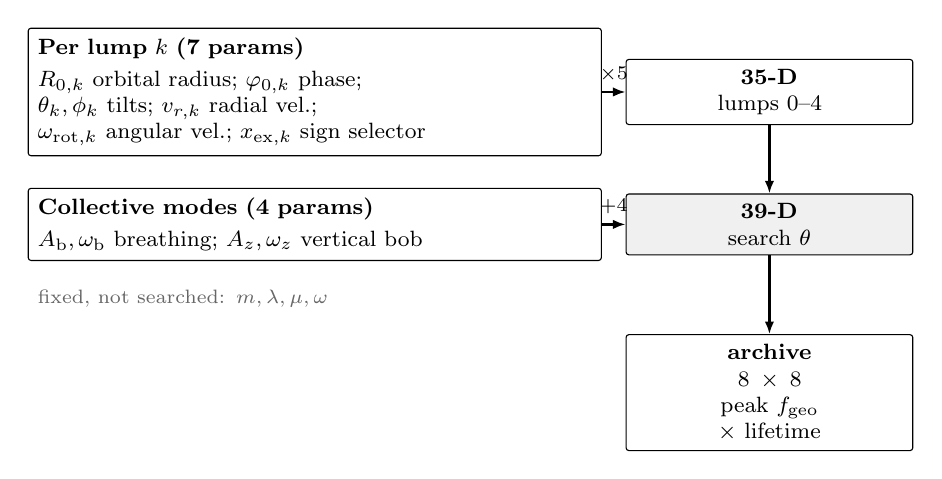
\begin{tikzpicture}[
  font=\footnotesize,
  box/.style={draw, rounded corners=1pt, align=center, inner sep=3.5pt},
  arr/.style={-{Latex[length=1.6mm]}, thick}
]
% --- column geometry: left stack + right totals ---
\node[box, align=left, text width=0.58\columnwidth] (lump) {%
  \textbf{Per lump $k$ (7 params)}\\[2pt]
  $R_{0,k}$ orbital radius;\ 
  $\varphi_{0,k}$ phase;\\
  $\theta_k,\phi_k$ tilts;\ 
  $v_{r,k}$ radial vel.;\\
  $\omega_{{\rm rot},k}$ angular vel.;\ 
  $x_{{\rm ex},k}$ sign selector};

\node[box, align=left, text width=0.58\columnwidth, below=4mm of lump] (coll) {%
  \textbf{Collective modes (4 params)}\\[2pt]
  $A_{\rm b},\omega_{\rm b}$ breathing;\ 
  $A_z,\omega_z$ vertical bob};

\node[below=2.5mm of coll, font=\scriptsize, text=black!60, align=left,
      text width=0.58\columnwidth] {%
  fixed, not searched: $m,\lambda,\mu,\omega$};

\node[box, right=3mm of lump, text width=0.28\columnwidth] (d35)
  {\textbf{35-D}\\lumps $0$--$4$};
\node[box, fill=black!6, right=3mm of coll, text width=0.28\columnwidth] (d39)
  {\textbf{39-D}\\search $\theta$};
\node[box, below=10mm of d39, text width=0.28\columnwidth] (arch)
  {\textbf{archive}\\$8\times8$\\peak $f_{\rm geo}$\\$\times$ lifetime};

\draw[arr] (lump.east) -- node[above, font=\scriptsize] {$\times 5$} (d35.west);
\draw[arr] (coll.east) -- node[above, font=\scriptsize] {$+4$} (d39.west);
\draw[arr] (d35.south) -- (d39.north);
\draw[arr] (d39.south) -- (arch.north);
\end{tikzpicture}
\caption{Search parameterization of the trajectory Q-ball shell:
$5\times7=35$ per-lump placement parameters plus 4 collective modes give the
$39$-D genome $\theta$. MAP-Elites stores one elite per cell of an
$8\times8$ archive indexed by peak shortcut and FTL lifetime. Q-ball
microphysics is held fixed.}
\label{fig:genome}
\end{figure}

\subsection{Lump orbit parameterization}
\label{sec:orbits}

Each lump moves in its own tilted orbital plane. The support center of lump $k$
is prescribed by
\begin{align}
r_k(t)&=\max\!\left[r_{\min},R_{0,k}+v_{r,k}t+
A_{\rm b}\sin(\omega_{\rm b}t)\right], \nonumber\\
\varphi_k(t)&=\varphi_{0,k}+\omega_{{\rm rot},k}t,\qquad
z_{\rm b}(t)=A_z\sin(\omega_z t),
\label{eq:lump_trajectory}
\end{align}
followed by rotation into the laboratory frame through the two tilt angles
$(\theta_k,\phi_k)$. Thus each lump spirals radially (drift $v_{r,k}$),
rotates in its own plane (angular velocity $\omega_{{\rm rot},k}$; negative
values are retrograde), and shares a collective radial breathing $(A_{\rm b},
\omega_{\rm b})$ and vertical oscillation $(A_z,\omega_z)$. The range of
possible orbits includes retrograde and prograde configurations, fast and slow
rotation, radially drifting spirals, and nearly static scaffolds.

\subsection{Trajectory controller (PD pump)}
\label{sec:pd_pump}

During evolution, a proportional--derivative (PD) controller drives the two
real components of each complex field toward a moving target profile at the
prescribed support center:
\begin{equation}
\begin{aligned}
\left.\partial_t\Pi_A\right|_{\rm PD}
  &=-w k_p(\phi_A-\phi_A^\star)\\
  &\quad-w k_d(\Pi_A-\Pi_A^\star),\qquad A=1,2 ,
\end{aligned}
\label{eq:pd_pump}
\end{equation}
with gains $k_p=12$, $k_d=7$, and $w$ the product of a localized envelope and
a constraint-sensitive governor. This is an external, non-Lagrangian source in
the scalar momentum equations; no corresponding pump stress-energy is added to
$T_{\mu\nu}$, so $\nabla_\mu T^{\mu\nu}=0$ is not exact while the pump is
active. The volume-integrated pump power
$P=\int\alpha\,(\Pi\cdot S_\Pi)\sqrt{\gamma}\,dV$ recorded in
\texttt{collapse\_diagnostics.dat} integrates to
$E_{\rm pump}\simeq1.6\times10^{-17}$ over the ignition window of the
pump-on HQ run---consistent with floating-point noise relative to the
matter amplitude ($|\phi|_{\rm max}\sim7\times10^{-2}$). The pump therefore
acts as a soft trajectory guide rather than a large energy injector. The
campaign default switches it off at $t_{\rm pump}=4$, and scoring credits
4D geodesic transport only for $t_{\rm emit}\ge t_{\rm pump}$, so the
headline geodesic---which launches at exactly $t_{\rm emit}=4$---samples a
freely evolved metric ($\nabla_\mu T^{\mu\nu}=0$). A dedicated pump-free HQ
twin with $t_{\rm pump}=0$ (Sec.~\ref{sec:pump_free}) tests whether the
shortcut survives with the PD term identically off from $t=0$.

\subsection{Constraint gate and source-model consistency}
\label{sec:selfconsistent}

A post-load constraint gate rejects inconsistent initial data before any GPU
time is spent: the solved data are loaded into \texttt{GRTeclyn} for a short
verification integration, and the volume-weighted $L^2$ constraint norms must
stay below a campaign threshold or the candidate is discarded and logged. The
bicomplex Q-ball campaigns use $3\times10^{-2}$ for the Hamiltonian and
$10^{-2}$ for the momentum residual; candidate~146 clears both comfortably at
$\|\mathcal H\|_2=5.9\times10^{-3}$ and
$\|\mathcal M\|_2=1.1\times10^{-4}$. This gate, together with bounded CCZ4
constraint growth, establishes numerical control and source-model consistency
for the \texttt{grtresna\_bicomplex\_scalar} model of
Sec.~\ref{sec:phantom_action}.

\subsection{Scoring: how every evaluation is rewarded}
\label{sec:scoring}

One fixed rule reduces every evaluation to a single fitness $S(\theta)$. Each
named quantity below is a normalized diagnostic in $[0,1]$ (penalties are
negative) and the score is their weighted sum,
\begin{align}
S =\;& 1000\,f_{\rm geo}^{\rm evol}
      + 1000\,f_{\rm geo}^{\rm op}
      + 600\,P_{\rm ftl}
      + 200\,F_{\rm op} \nonumber\\
   &  + 200\,C_{\rm curv}
      + 5\,G_{\rm nt}
      + g_{\rm h}\,\Sigma_{\rm health}\nonumber\\
   &  + 40\,w_{x}\,X_{\rm exotic}
      + 200\,H_{\rm hor},
\label{eq:score}
\end{align}
with the health block
\begin{equation}
\Sigma_{\rm health}=150\,\mathrm{surv}+60\,E+40\,\mathrm{stab}
+30\,\mathrm{cmv}+10\,\mathcal H_{\rm ok}+15\,I,
\end{equation}
gated by the nontriviality factor $g_{\rm h}\in[0,1]$ so that a flat
configuration earns no health reward. Inside the score the raw advantage
$f_{\rm geo}$ is mapped to a saturating magnitude
$\hat f=\min\!\bigl[(f_{\rm geo}-10^{-3})/(0.2-10^{-3}),\;1\bigr]$, so marginal
shortcuts earn proportionally less and full marks require
$f_{\rm geo}\ge20\%$; the two geodesic slots then pay $1000\,\hat f\,p_{\rm s}$
with $p_{\rm s}$ the structural persistence (density retention $\times$
coherence $\times$ confinement). Whenever a 4D evolving trace exists it takes
precedence: the frozen slot is zeroed, $f_{\rm geo}^{\rm op}\equiv0$, so the two
$1000$-weight terms are mutually exclusive rather than additive.
Table~\ref{tab:weights} lists what each
term measures. Two design choices matter. First, transport dominates and every
transport-flavored term---$f_{\rm geo}^{\rm evol}$, $P_{\rm ftl}$, and
$F_{\rm op}$---is multiplied by the fraction of matter still confined, so no
candidate can bank a coordinate superluminal channel after its lumps have flown
apart. Second, the exotic penalty $X_{\rm exotic}<0$ charges for
energy-condition violation~\cite{le2026warpax} but is deliberately weak: at the
campaign value $w_x=0.2$ and the graded floor $X_{\rm exotic}\ge-1.6$ it reaches
at most ${\approx}13$ points against the ${\approx}417$ the champion earns from
the persistence-gated geodesic term. The optimizer may therefore spend exotic
matter freely in exchange for genuine transport, which is why the archive
populates the phantom sector rather than being pinned to $X_{\rm exotic}=0$.
Search-tier scores are values of $S$ on a $t=16$ evolution
(Sec.~\ref{sec:stages}); the only production $S$ values appear in the
pump-free comparison (Table~\ref{tab:pump_compare}). For the CMA-ES champion
(candidate~146) the search-tier score is $S=852.15$
(Sec.~\ref{sec:methodology}).

\begin{table}[tbp]
\caption{Reward terms in the campaign objective [Eq.~\eqref{eq:score}], applied
identically to every MAP-Elites evaluation.}
\label{tab:weights}
\begin{ruledtabular}
\begin{tabular}{llr}
symbol & rewards / penalizes & weight \\
\hline
$f_{\rm geo}^{\rm evol}$ & 4D evolving null shortcut & $1000$ \\
$f_{\rm geo}^{\rm op}$ & geodesic (frozen) shortcut & $1000$ \\
$P_{\rm ftl}$ & FTL persistence (gated) & $600$ \\
$F_{\rm op}$ & operational coord.\ FTL (gated) & $200$ \\
$C_{\rm curv}$ & curvature activity & $200$ \\
$G_{\rm nt}$ & nontrivial geometry & $5$ \\
$\mathrm{surv}$ & structural survival & $150\,g_{\rm h}$ \\
$E$ & energy-condition health & $60\,g_{\rm h}$ \\
$\mathrm{stab}$ & metric stability & $40\,g_{\rm h}$ \\
$\mathrm{cmv}$ & co-moving stability & $30\,g_{\rm h}$ \\
$I$ & instability penalty & $15\,g_{\rm h}$ \\
$\mathcal H_{\rm ok}$ & constraint health & $10\,g_{\rm h}$ \\
$X_{\rm exotic}$ & exotic-matter penalty & $40\,w_{x}$ \\
$H_{\rm hor}$ & horizon-formation penalty & $200$ \\
\end{tabular}
\end{ruledtabular}
\end{table}

\subsection{Search and validation stages}
\label{sec:stages}

MAP-Elites and CMA-ES evaluate $\mathcal{O}(10^2)$ genomes, so the discovery
loop uses a reduced GRTeclyn configuration for wall-clock speed
(Table~\ref{tab:search_vs_hq_grid}). Archive and CMA scores are therefore
\emph{search-tier} diagnostics, not continuum claims; only the frozen champion
is re-run at production resolution. The campaign ladder
(Fig.~\ref{fig:campaign-stages}) has four stages.

\begin{itemize}
    \item \textbf{Stage 1 --- MAP-Elites discovery.} Quality-diversity search
    on the search grid, with per-lump gravitational signs retained in
    evolution. The coarse AMR is intentional: it buys enough evaluations to
    fill the behavior archive.
    \item \textbf{Stage 2 --- CMA-ES refinement.} Warm-start from the
    MAP-Elites champion and its nearest elites; local covariance-matrix
    adaptation at the \emph{same} grid, $t_{\rm stop}$, and scoring rule. Only
    the refined top genome is promoted.
    \item \textbf{Stage 3 --- production replay (HQ).} The frozen champion is
    re-solved and evolved at higher fidelity and longer $t_{\rm stop}$, with
    multiple emission times and multi-ray geodesic probes. Every headline
    number in this paper comes from here, not from MAP-Elites.
    \item \textbf{Stage 4 --- resolution and domain matrix.} Matched
    coarse/medium/fine runs (RC/RM/RF at fixed $L=128$, $N=192/256/384$) test
    continuum stability; matched-spacing domain runs (DS/DL at $h=0.500$,
    $L=96/160$) test boundary sensitivity on the same $t_{\rm stop}$ window.
\end{itemize}

\begin{table}[tbp]
\caption{GRTeclyn evolution settings: search tier (MAP-Elites / CMA-ES)
versus production validation (HQ / Richardson medium). Search uses a
reduced grid for throughput; validation upgrades $L$, $N$,
\texttt{max\_level}, and $t_{\rm stop}$.
Campaign env:
\texttt{GRTRESNA\_EVOLUTION\_\{L,N\}\_FULL},
\texttt{\_MAX\_LEVEL},
\texttt{\_REGRID\_THRESHOLD}.}
\label{tab:search_vs_hq_grid}
\begin{ruledtabular}
\begin{tabular}{lcc}
parameter & search & HQ / RM \\
\hline
$L$ & $64$ & $128$ \\
$N$ & $128$ & $256$ \\
$h=L/N$ & $0.5$ & $0.5$ \\
\texttt{max\_level} & $1$ & $3$ \\
\texttt{regrid\_threshold} & $0.1$ & $0.02$ \\
$t_{\rm stop}$ & $16$ & $30$ \\
\end{tabular}
\end{ruledtabular}
\end{table}

\begin{figure}[tbp]
\centering
\resizebox{0.98\columnwidth}{!}{%
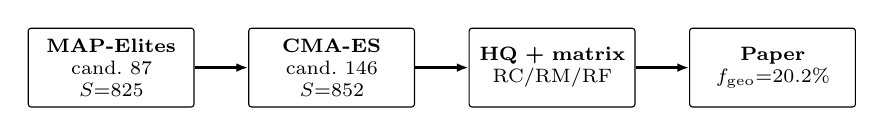
\begin{tikzpicture}[
  font=\scriptsize,
  box/.style={draw, rounded corners=1pt, align=center,
              text width=20mm, minimum height=10mm, inner sep=1.5pt},
  flow/.style={-{Latex[length=1.5mm]}, thick}
]
\node[box] (me) at (0,0) {\textbf{MAP-Elites}\\cand.~87\\$S{=}825$};
\node[box] (cma) at (2.8,0) {\textbf{CMA-ES}\\cand.~146\\$S{=}852$};
\node[box] (hq) at (5.6,0) {\textbf{HQ + matrix}\\RC/RM/RF};
\node[box] (paper) at (8.4,0) {\textbf{Paper}\\$f_{\rm geo}{=}20.2\%$};
\draw[flow] (me)--(cma);
\draw[flow] (cma)--(hq);
\draw[flow] (hq)--(paper);
\end{tikzpicture}}
\caption{Outer campaign ladder. MAP-Elites finds the diverse archive and
champion (87); CMA-ES refines it to candidate~146; only the refined champion
enters high-resolution replay and the resolution matrix.}
\label{fig:campaign-stages}
\end{figure}

\begin{figure*}[tbp]
\centering
\resizebox{0.94\textwidth}{!}{%
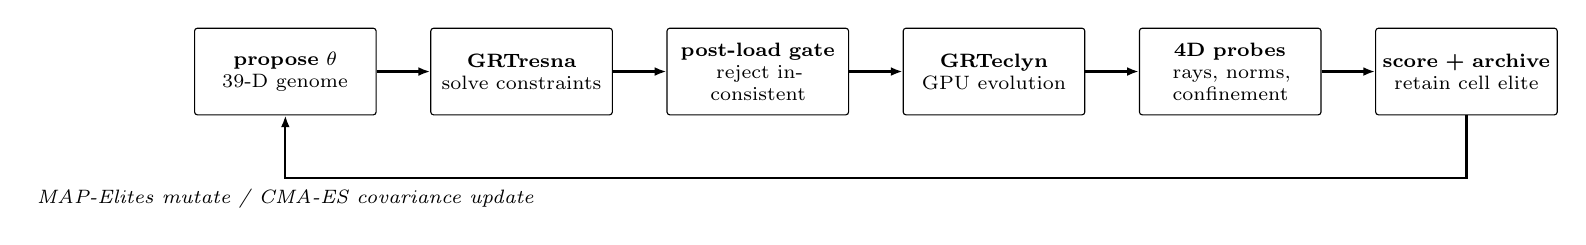
\begin{tikzpicture}[
  font=\scriptsize,
  box/.style={draw, rounded corners=1pt, align=center,
              text width=22mm, minimum height=11mm, inner sep=1.5pt},
  flow/.style={-{Latex[length=1.5mm]}, thick}
]
\node[box] (proposal) at (0,0) {\textbf{propose $\theta$}\\39-D genome};
\node[box] (solve) at (3.0,0) {\textbf{GRTresna}\\solve constraints};
\node[box] (gate) at (6.0,0) {\textbf{post-load gate}\\reject inconsistent};
\node[box] (evolve) at (9.0,0) {\textbf{GRTeclyn}\\GPU evolution};
\node[box] (probe) at (12.0,0) {\textbf{4D probes}\\rays, norms, confinement};
\node[box] (archive) at (15.0,0) {\textbf{score + archive}\\retain cell elite};
\draw[flow] (proposal)--(solve);
\draw[flow] (solve)--(gate);
\draw[flow] (gate)--(evolve);
\draw[flow] (evolve)--(probe);
\draw[flow] (probe)--(archive);
\draw[flow] (archive.south) -- ++(0,-8mm) -|
  node[pos=0.50, below, font=\scriptsize\itshape]
  {MAP-Elites mutate / CMA-ES covariance update} (proposal.south);
\end{tikzpicture}}
\caption{Inner evaluation loop shared by MAP-Elites and CMA-ES. Failed
constraint solves and post-load checks never enter GPU evolution; successful
evaluations compete for archive cells (MAP-Elites) or update the CMA
distribution.}
\label{fig:pipeline}
\end{figure*}

\section{Search Methodology}
\label{sec:methodology}

\subsection{MAP-Elites quality-diversity}

MAP-Elites~\cite{mouret15} is a quality-diversity search: instead of returning
one champion, it maintains an $8\times8$ archive with at most one elite per
behavior cell. A candidate displaces the occupant of its cell only if its score
$S(\theta)$ [Eq.~\eqref{eq:score}] is higher. The two archive axes are peak
shortcut strength and FTL lifetime, so the campaign can keep short-lived strong
channels and longer weaker ones side by side. The bicomplex campaign
scheduled 200 evaluations: 148 completed GPU evolution, 50 failed the post-load
gate, one failed the GRTresna admission gate, and one failed the constraint
solve. The best score rose from $690.1$ to $825.19$ and last improved at
batch~10, when candidate~87 entered the strongest cell
(Fig.~\ref{fig:search_progress}a). The fixed $200$-evaluation budget is
set to outlast saturation---termination requires a plateaued archive-best score
and static cell coverage---and here both stall by batch~10, so the budget and
the saturation criterion coincide.

Nine of the $64$ cells ended occupied ($14.06\%$ coverage): all eight bins of
the strength axis in the highest-lifetime row, plus one zero-lifetime cell. The
archive is therefore a clean strength ladder---peak $f_{\rm geo}$ climbs from
$1.8\%$ to $25.4\%$ while every elite holds its channel open for the full
scored window---and score broadly tracks it, because transport carries the
$1000$-weight terms of Eq.~\eqref{eq:score} and nothing else in the objective
comes close. What score does \emph{not} track is persistence, which wanders
between $27.8\%$ and $39.6\%$ with no trend along the ladder---the first sign
that strength and confinement are set by different features of the genome.

\begin{figure}[tbp]
\centering
\begin{tikzpicture}
\begin{axis}[
  width=0.94\columnwidth,
  height=0.45\columnwidth,
  xlabel={MAP-Elites batch (8 evaluations)},
  ylabel={best score},
  xmin=0,xmax=25,
  ymin=650,ymax=860,
  xtick={0,5,10,15,20,25},
  ytick={650,700,750,800,850},
  grid=major,grid style={gray!18},
  tick label style={font=\small},
  label style={font=\small},
  title={\small (a) MAP-Elites}
]
\addplot[black,very thick,mark=*,mark size=1.8pt]
  table[x=batch,y=best]{data/campaign_progress.txt};
\addplot[only marks,mark=square*,mark size=3pt]
  coordinates {(10,825.194)};
\node[anchor=north west,font=\scriptsize] at (axis cs:10.2,820)
  {champion: $825.19$};
\end{axis}
\end{tikzpicture}

\vspace{0.3cm}

\begin{tikzpicture}
\begin{axis}[
  width=0.94\columnwidth,
  height=0.45\columnwidth,
  xlabel={CMA-ES evaluation},
  ylabel={running best score},
  xmin=0,xmax=150,
  ymin=820,ymax=862,
  ytick={820,830,840,850,860},
  grid=major,grid style={gray!18},
  tick label style={font=\small},
  label style={font=\small},
  title={\small (b) CMA-ES refinement}
]
\addplot[black,very thick]
  table[x=eval,y=best]{data/cmaes_progress.txt};
\addplot[gray,dashed,thick,domain=0:150]{825.194};
\node[anchor=north west,font=\scriptsize,text=gray,fill=white,inner sep=1pt]
  at (axis cs:3,824.6)
  {ME baseline: $825.19$};
\addplot[only marks,mark=square*,mark size=3pt,red]
  coordinates {(146,852.145)};
\node[anchor=north east,font=\scriptsize,text=red,fill=white,inner sep=1pt]
  at (axis cs:143,859.5)
  {CMA champion: $852.15$};
\end{axis}
\end{tikzpicture}
\caption{Search progress.
(a)~MAP-Elites running best score over 200 evaluations; the champion
(candidate~87) enters cell $(7,7)$ at batch~10 with $S=825.19$.
(b)~CMA-ES refinement over 150 evaluations, warm-started from
MAP-Elites champion~87; dashed line marks the MAP-Elites best ($825.19$);
the running best reaches $852.15$ at candidate~146.}
\label{fig:search_progress}
\end{figure}

\subsection{The strongest shortcut is not the promoted one}
\label{sec:strength_vs_persistence}

Neither champion is the largest shortcut its stage produced
(Table~\ref{tab:strength_persistence}). The strongest evolving advantage
anywhere in the MAP-Elites run is $34.56\%$ (eval~99), nine percentage points
above the archive champion; the strongest in the whole study is $39.46\%$
(CMA-ES eval~136), nearly double candidate~146. Both were rejected by the same
mechanism. Eval~99 retained $9.7\%$ of its matter and eval~136 $22.5\%$, against
$39.6\%$ and $41.7\%$ for the promoted genomes, and because every
transport-flavored term in Eq.~\eqref{eq:score} is multiplied by that retained
fraction, their scores land at $314$ and $534$ instead of $825$ and $852$. The
gate is doing exactly what Sec.~\ref{sec:scoring} designed it to do: a large
$f_{\rm geo}$ measured while the source is flying apart buys almost nothing.

\begin{table}[tbp]
\caption{Strongest raw shortcut of each search stage against the genome
actually promoted. The first four rows are search tier, the last is the
production replay; persistence is the confinement-gated structural
persistence. The promoted champions are weaker and better confined.}
\label{tab:strength_persistence}
\begin{ruledtabular}
\begin{tabular}{llrrr}
stage & role & $f_{\rm geo}$ & persist. & $S$ \\
\hline
MAP-Elites & strongest (99)     & $34.56\%$ & $9.7\%$  & $314.0$ \\
MAP-Elites & champion (87)      & $25.35\%$ & $39.6\%$ & $825.2$ \\
CMA-ES     & strongest (136)    & $39.46\%$ & $22.5\%$ & $534.3$ \\
CMA-ES     & champion (146)     & $20.12\%$ & $41.7\%$ & $852.1$ \\
HQ RM      & replay of 146      & $20.21\%$ & ---      & --- \\
\end{tabular}
\end{ruledtabular}
\end{table}

The trade is systematic, not anecdotal. Over the $119$ MAP-Elites evaluations
with $f_{\rm geo}>0$, strength and persistence are anti-correlated
($r=-0.15$), and their strongest quartile averages $27.3\%$ persistence against
$31.0\%$ for the weakest; the $141$ such CMA-ES evaluations are more strongly
anti-correlated still ($r=-0.32$). Reading down
Table~\ref{tab:strength_persistence}, the campaign is
already sketching the same Pareto frontier the geometry-first atlas maps
kinematically in Sec.~\ref{sec:geometry_ceiling}: the configurations that open
the widest channel are the ones least able to hold it open.

\subsection{CMA-ES refinement and the promotion of candidate~146}

CMA-ES warm-started from candidate~87 and ran 150 evaluations (144 GPU-ok) at
the same search grid, reaching $S=852.15$ at candidate~146
($\Delta S\approx+27$; Fig.~\ref{fig:search_progress}b). The gain is
\emph{entirely} on the persistence side: the search-tier $f_{\rm geo}$
\emph{fell} from $25.35\%$ to $20.12\%$ while structural persistence rose from
$39.6\%$ to $41.7\%$. CMA-ES bought that by collapsing onto a quasi-static
scaffold---all five angular velocities below $5\times10^{-3}$ and breathing
amplitude $0.083$---which keeps the lumps in place long enough for the gated
terms to pay out. The run is converged rather than merely lucky: the eight
best genomes all sit at $f_{\rm geo}=19.9$--$20.4\%$ and persistence
$41.5$--$41.7\%$, within $4$ points of score of each other, so candidate~146
is the representative of a stable basin and not an isolated spike.

Candidate~146 then goes to production replay, where the $L=128$, $N=256$
evolution reproduces the search-tier shortcut at $20.21\%$ with all five rays
reaching---agreement to $0.5\%$ relative across a doubling of resolution and a
tripling of refinement depth. Its $41.7\%$ retention, however, is measured at
$t=16$, and the production window runs to $t=30$: the longer integration
stresses persistence much harder (Sec.~\ref{sec:dispersion}).

\section{Diagnostics and Probe Validation}
\label{sec:probes}

\subsection{The 4D evolving null-geodesic trace}

The transport claim rests on tracing light rays through the simulated
spacetime, not on reading coordinate speeds off a slice. A coordinate
operational shortcut $F_{\rm op}$ [Eq.~\eqref{eq:f_op}] can flag tilted light
cones, but it is partly gauge dependent and can be inflated by a coordinate
choice. The authoritative probe therefore integrates the null-geodesic
equations
\begin{equation}
\dot x^\mu=g^{\mu\nu}k_\nu, \qquad \dot k_\mu=-\tfrac12(\partial_\mu g^{\alpha\beta}) k_\alpha k_\beta,
\label{eq:geodesic_eqs}
\end{equation}
for a photon with position $x^\mu$ and momentum $k_\mu$. ``4D'' means the ray
is not confined to one snapshot: it is pushed through a stack of stored time
slices, so at each step the metric $g_{\mu\nu}(t,\mathbf{x})$ used is the one
that actually exists when the photon is at that point. This distinguishes it
from a \emph{frozen} trace, which wrongly assumes a single slice persists for
the whole flight.

The construction is as follows. A ray is emitted at time $t_{\rm emit}$ from a
fixed source point toward a fixed receiver. The quantities that enter the
shortcut formulas are \emph{transit durations}, not absolute grid arrival
times: $t_B^{\rm curved}$ (respectively $t_{\rm min}$) is the coordinate time
elapsed along the curved path after emission, and $t_B^{\rm flat}$
(respectively $t_{\rm flat}$) is the matched flat-space flight duration between
the same endpoints. Absolute arrival on the grid is
$t_{\rm arrival}=t_{\rm emit}+t_B^{\rm curved}$. The fractional advantage is
\begin{equation}
F_{\rm op}=\frac{t_B^{\rm flat}-t_B^{\rm curved}}{t_B^{\rm flat}},
\label{eq:f_op}
\end{equation}
\begin{equation}
f_{\rm geo}=\max\!\left(0,\;\frac{t_{\rm flat}-t_{\rm min}}{t_{\rm flat}}\right),
\label{eq:f_geo}
\end{equation}
so $f_{\rm geo}=0$ means no shortcut. A launch is accepted only if its rays
stay physical: the relative drift in the null Hamiltonian
$g^{\mu\nu}k_\mu k_\nu=0$ must remain below $10^{-2}$, which rejects rays that
have accumulated interpolation error. Because a ray needs a long remaining
segment of evolved geometry to reach the far endpoint (flat transit is
$t_{\rm flat}=14.4$) while the metric stack ends at $t=30$, late launches
cannot finish a fair comparison. We therefore sweep seven early launch times,
$t_{\rm emit}=0,2,\ldots,12$ (five rays each), and report the largest accepted
$f_{\rm geo}$. Across the pump-on validation matrix the peak sits at
$t_{\rm emit}=4$, just after the PD pump switches off, and has fallen to zero
by $t_{\rm emit}=12$, so the window brackets the full life of the channel. (In
the pump-free twin the optimum sits at the edge of the same window;
Sec.~\ref{sec:pump_free}.)

\subsection{Freely falling observer timing metric}
\label{sec:freefall_metric}

As a stronger complement to the fixed-plane coordinate diagnostic
$f_{\rm geo}$, we define an observer-to-observer timing metric. At the initial
slice, an emitter $A$ and receiver $B$ are placed at the central source and
detector locations used by the null-ray probe and are released with four-velocity
equal to the future-directed Eulerian normal $n^\mu$. Their worldlines
$\gamma_A$ and $\gamma_B$ are then evolved as timelike geodesics,
\begin{equation}
\frac{dx^\mu}{d\tau}=g^{\mu\nu}p_\nu,\qquad
\frac{dp_\mu}{d\tau}
=-\frac{1}{2}\partial_\mu g^{\alpha\beta}p_\alpha p_\beta,\qquad
g^{\mu\nu}p_\mu p_\nu=-1,
\label{eq:timelike_observers}
\end{equation}
where $\tau$ is the observer's proper time. Emission is scheduled by the
emitter's clock, $\tau_A=\tau_{\rm emit}$, rather than by simulation coordinate
time. At the emission event, an orthonormal spatial triad
$e_{(a)}{}^\mu$ is constructed in the emitter's rest frame and the photon wave
vector is launched as
\begin{equation}
k^\mu=u_A^\mu+\hat n^a e_{(a)}{}^\mu,\qquad
\delta_{ab}\hat n^a\hat n^b=1,
\label{eq:freefall_null_launch}
\end{equation}
up to an irrelevant positive affine rescaling. The two launch angles and the
arrival affine parameter are solved simultaneously so that the ray intersects
the moving receiver worldline $\gamma_B$: reception is a worldline event, not
the crossing of a coordinate detector plane. The physical miss distance
$\delta_B=(\gamma_{ij}\Delta x^i\Delta x^j)^{1/2}$ at the candidate event is
retained as a quality diagnostic alongside the null and timelike mass-shell
residuals.

For the matched Minkowski experiment, the two inertial observers are initially
comoving, their clocks are synchronized on the reference initial slice, and
their separation is the initial proper length
\begin{equation}
D_0=\int_A^B\sqrt{\gamma_{ij}\,dx^i dx^j}.
\label{eq:freefall_initial_separation}
\end{equation}
The flat receiver therefore records
$\tau_{B,\rm flat}=\tau_{\rm emit}+D_0$, and if the curved reception event
occurs at receiver proper time $\tau_{B,\rm curved}$ the metric is
\begin{equation}
f_{\rm ff}
=\frac{\tau_{B,\rm flat}-\tau_{B,\rm curved}}
       {D_0}.
\label{eq:freefall_metric}
\end{equation}
A positive $f_{\rm ff}$ means the freely falling receiver records the photon
earlier than in the matched flat experiment. Absorbing endpoint lapse, shift,
clock rate, and receiver motion into the measured worldlines makes this less
coordinate-conditioned than Eq.~\eqref{eq:f_geo}, though not fully gauge
invariant: the initial slice and the endpoint-selection prescription remain
part of the operational definition.

\begin{figure}[tbp]
\centering
\resizebox{0.98\columnwidth}{!}{%
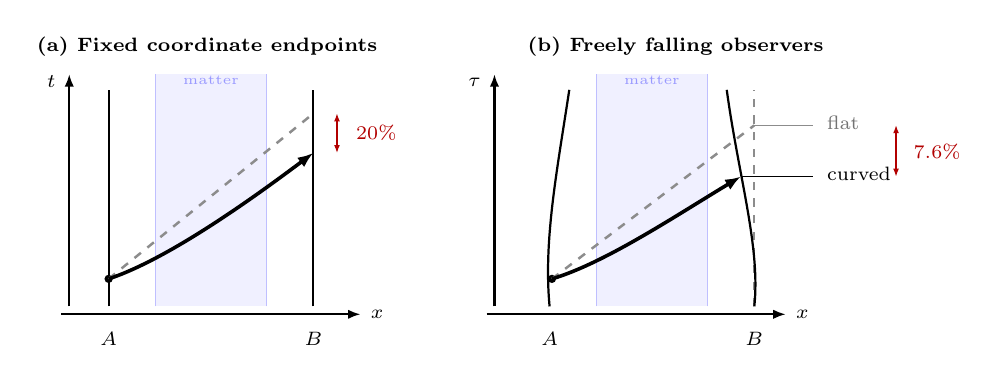
\begin{tikzpicture}[>=Latex, font=\scriptsize]
% --- Symbolic x axes for each panel ---
\draw[-{Latex[length=1.6mm]}, thick] (0.00,0.45) -- (3.80,0.45)
  node[right] {$x$};
\draw[-{Latex[length=1.6mm]}, thick] (5.40,0.45) -- (9.20,0.45)
  node[right] {$x$};
% --- Panel (a): fixed coordinate endpoints ---
\node[font=\scriptsize\bfseries] at (1.85,3.85)
  {(a) Fixed coordinate endpoints};
% Matter region band (behind everything)
\fill[blue!6] (1.20,0.55) rectangle (2.60,3.50);
\draw[blue!25] (1.20,0.55) -- (1.20,3.50);
\draw[blue!25] (2.60,0.55) -- (2.60,3.50);
\node[blue!40, font=\tiny] at (1.90,3.42) {matter};
\draw[-{Latex[length=1.6mm]}, thick] (0.10,0.55) -- (0.10,3.50);
\node[anchor=east] at (0.05,3.40) {$t$};
\draw[thick] (0.60,0.55) -- (0.60,3.30);
\draw[thick] (3.20,0.55) -- (3.20,3.30);
\node[below] at (0.60,0.35) {$A$};
\node[below] at (3.20,0.35) {$B$};
\fill (0.60,0.90) circle (1.5pt);
\draw[black!45, dashed, line width=0.9pt]
  (0.60,0.90) -- (3.20,3.00);
\draw[black, line width=1.3pt, -{Latex[length=2mm]}]
  (0.60,0.90) .. controls (1.35,1.15) and (2.40,1.90) .. (3.20,2.50);
\draw[{Latex[length=1mm]}-{Latex[length=1mm]}, red!70!black]
  (3.50,2.50) -- (3.50,3.00);
\node[red!70!black, anchor=west] at (3.62,2.75)
  {$20\%$};

% --- Panel (b): freely falling observers ---
\node[font=\scriptsize\bfseries] at (7.80,3.85)
  {(b) Freely falling observers};
% Matter region band
\fill[blue!6] (6.80,0.55) rectangle (8.20,3.50);
\draw[blue!25] (6.80,0.55) -- (6.80,3.50);
\draw[blue!25] (8.20,0.55) -- (8.20,3.50);
\node[blue!40, font=\tiny] at (7.50,3.42) {matter};
\draw[-{Latex[length=1.6mm]}, thick] (5.50,0.55) -- (5.50,3.50);
\node[anchor=east] at (5.45,3.40) {$\tau$};
% Emitter worldline (slightly curved, thick)
\draw[thick]
  (6.20,0.55) .. controls (6.12,1.40) and (6.30,2.30) .. (6.45,3.30);
\node[below] at (6.20,0.35) {$A$};
% Receiver: inertial reference (dashed vertical, same start)
\draw[thick, black!45, dashed] (8.80,0.55) -- (8.80,3.30);
% Receiver: actual curved worldline (solid, drifts left)
\draw[thick]
  (8.80,0.55) .. controls (8.88,1.30) and (8.60,2.20) .. (8.45,3.30);
\node[below] at (8.80,0.35) {$B$};
% Emission event
\fill (6.23,0.90) circle (1.5pt);
% Dashed flat ray hits inertial receiver (arrives later)
\draw[black!45, dashed, line width=0.9pt]
  (6.23,0.90) -- (8.80,2.85);
% Solid curved ray hits curved receiver (arrives earlier)
\draw[black, line width=1.3pt, -{Latex[length=2mm]}]
  (6.23,0.90) .. controls (6.90,1.10) and (7.80,1.70) .. (8.63,2.20);
% Arrival markers on right margin
\draw[black, thin] (8.63,2.20) -- (9.55,2.20);
\draw[black!45, thin] (8.80,2.85) -- (9.55,2.85);
\node[anchor=west] at (9.60,2.20) {\strut curved};
\node[anchor=west, black!55] at (9.60,2.85) {\strut flat};
% Bracket for advantage (far right)
\draw[{Latex[length=1mm]}-{Latex[length=1mm]}, red!70!black]
  (10.60,2.20) -- (10.60,2.85);
\node[red!70!black, anchor=west] at (10.70,2.52)
  {$7.6\%$};
\end{tikzpicture}}
\caption{Two operational measurements of the same candidate~146 (RM).
(a)~Fixed endpoints: dashed = flat ray, solid = curved ray arriving $20\%$
earlier at fixed~$B$.
(b)~Free-fall observers: both receivers start at~$B$; the solid worldline
drifts in curved spacetime while the dashed one stays inertial. The solid
photon hits the curved receiver earlier (``curved'') than the dashed photon
hits the inertial one (``flat''). The $7.6\%$ bracket is the proper-time
advance. The two protocols differ in what they measure, not in candidate
quality.}
\label{fig:timing_protocols}
\end{figure}

For candidate~146 in the corrected RM replay, the fixed-endpoint probe gives
$f_{\rm geo}\simeq20\%$, whereas the freely falling protocol gives
$f_{\rm ff}=7.62\%$: $D_0=13.851$, $\tau_{B,\rm flat}=17.851$, and
$\tau_{B,\rm curved}=16.796$, so the receiver-clock advance is $1.055$ and
$f_{\rm ff}=1.055/13.851=7.62\%$. The smaller magnitude is not a degradation of
the candidate. The two protocols measure different things
(Fig.~\ref{fig:timing_protocols}): releasing the endpoints changes the
reception event, and proper-time readout absorbs their motion and accumulated
clock rates. Which piece of geometry accounts for the difference is settled
quantitatively in Sec.~\ref{sec:mechanism}. Normalizing by $D_0$ rather than by
the absolute clock reading $\tau_{B,\rm flat}$ makes the fraction independent
of an arbitrary common shift of the clocks' zero.

Moving-puncture coordinates are prone to slice stretching, so it matters that
this protocol never leaves the weak field. Both $A$ and $B$ start in the
near-flat region (Table~\ref{tab:endpoint_gauge}) and are released with
Eulerian normal four-velocity; the reported quantity is the receiver's own
proper time at a reception event on its own worldline, normalized by an
initial proper length. The $7.6\%$ advance is therefore physically unambiguous
in a way the coordinate figure is not.

\subsection{Null-constraint accuracy along the flight path}
\label{sec:null_accuracy}

The $10^{-2}$ acceptance gate is a conservative safety bound, not the achieved
accuracy. Two mechanisms keep the ray far tighter. First, whenever the absolute
null Hamiltonian exceeds $10^{-6}$ the momentum is re-projected onto the local
null cone before the next Runge--Kutta step, so interpolation error cannot
accumulate secularly. Second, the normalized null constraint stays small between
projections. Along the headline candidate-146 ray ($t_{\rm emit}=4$,
RM), the gauge-independent ratio $k_\mu k^\mu/(k^t)^2$ has median
$3.0\times10^{-4}$ (a factor ${\sim}30$ below the gate) and a brief peak of
$4.1\times10^{-3}$ in the strong-field core (still a factor ${\sim}2.4$ under
the gate). The ray therefore stays null to the stated tolerance throughout and
does not drift toward a timelike or spacelike trajectory. The complementary
relative-drift diagnostic recorded by the probe,
$h_{\rm rel}^{\rm max}=2.19\times10^{-3}$ in RM, tells the same story.

\subsection{Probe controls and calibration}

Three controls bracket the probe's dynamic range before any candidate is
evaluated.
\begin{itemize}
  \item \textbf{Minkowski (flat):} $f_{\rm geo}=0$ by construction; verifies
    that the tracer introduces no spurious shortcut on trivial data.
  \item \textbf{Prescribed Alcubierre}~\cite{alcubierre94}\textbf{:} a
    moving-bubble metric ($v_s=0.5$, bubble radius~$2$, wall width~$2$) is
    built analytically and fed to the evolving tracer, yielding
    $f_{\rm geo}\approx32\%$ with $5/5$ rays reaching. This confirms
    that the 4D probe recovers a known coordinate shortcut.
  \item \textbf{Negative control (eval\,086):} an earlier campaign candidate
    whose frozen-slice diagnostic shows $f_{\rm geo}\approx5.8\%$, but whose
    4D evolving HQ trace collapses to $0\%$ ($0/5$ rays). This false positive
    motivated the design rule that the evolving trace is authoritative: frozen
    peaks alone do not certify transport.
\end{itemize}
The positive campaign control is the CMA-ES champion (candidate~146): every
accepted launch in all three resolution-matrix runs has $5/5$ rays reaching
and passes the null-Hamiltonian gate.

\section{Results: Candidate-146 Warp Precursor}
\label{sec:results}

\subsection{Provenance and genome}

Candidate~146 is the CMA-ES-refined champion from the bicomplex campaign
(Sec.~\ref{sec:methodology}). Its provenance freezes the exact
39-dimensional genome, source checksums, solver parameters, and source
commit. The finest run (RF) additionally stored field maps, from which the
snapshots of Fig.~\ref{fig:rf_field_maps} are drawn.

\subsection{Matter dynamics}

Candidate~146 uses five lumps with source signs
$s_k=(+1,-1,-1,+1,-1)$ (two canonical, three phantom;
Sec.~\ref{sec:phantom_action}).
The collective breathing is small ($A_{\rm b}=0.083$,
$\omega_{\rm b}=0.429$), the vertical oscillation is moderate ($A_z=2.32$,
$\omega_z=0.016$), and the initial radii are
$R_0=(3.69,5.50,2.83,5.59,2.61)$. All angular velocities are negative,
$\omega_{\rm rot}=(-0.0017,-0.0007,-0.0031,-0.0009,-0.0049)$, so all five
trajectories are retrograde but extremely slow. Radial drifts are small
[$v_r=(-0.060,-0.010,\,0.001,-0.005,-0.006)$] and roughly an order of
magnitude quieter than MAP-Elites champion~87, the quasi-static scaffold
CMA-ES converged to (Sec.~\ref{sec:methodology}).

The PD trajectory controller (Sec.~\ref{sec:pd_pump}) drives the lumps during
the ignition phase ($t<4$) and then switches off; the evolution remains
numerically controlled throughout (Fig.~\ref{fig:constraints}).
Figure~\ref{fig:lump_topdown} shows an unscaled top-down ($x$--$y$) projection
confirming that the shell spans only a few code units across the null-probe
corridor. Those support centers are the intended dynamical scaffold, not
tracked density isosurfaces, and the field follows them imperfectly:
confinement falls from $72\%$ to $11\%$ and rms spread grows by a factor $3.27$
by $t=30$. Candidate~146 is a transient, initially driven configuration, not a
bound five-body soliton.


\begin{figure}[tbp]
\centering
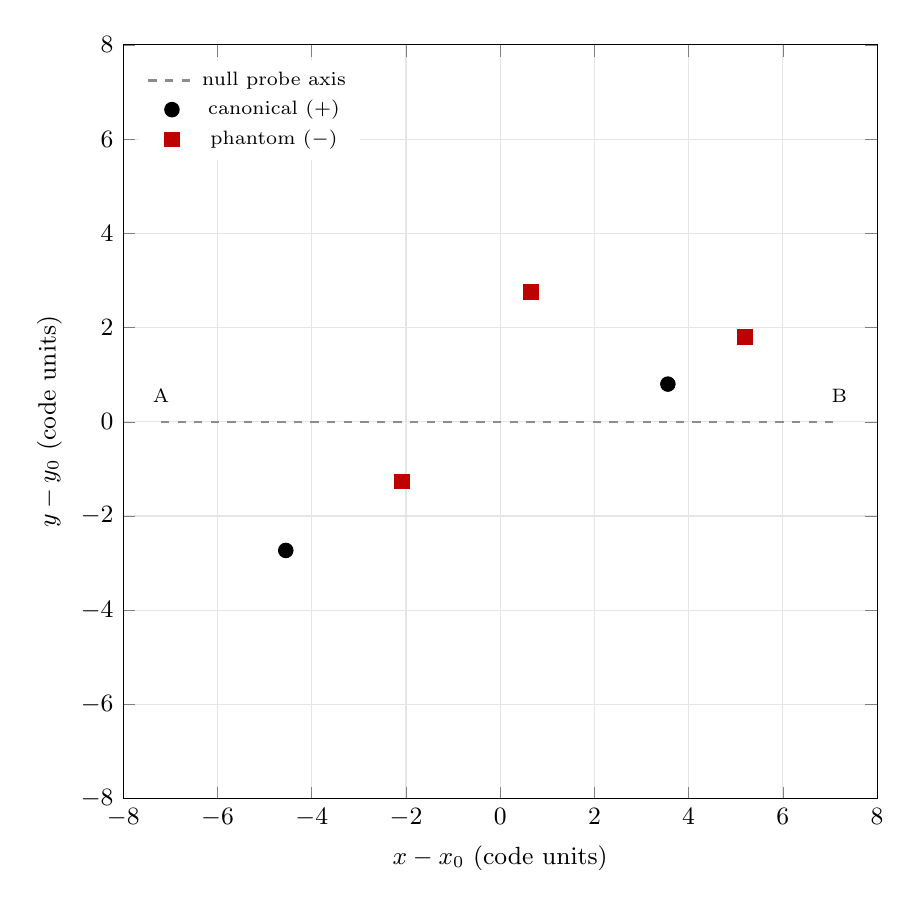
\begin{tikzpicture}
\begin{axis}[
  width=0.92\columnwidth,height=0.92\columnwidth,
  axis equal image,
  xlabel={$x-x_0$ (code units)},ylabel={$y-y_0$ (code units)},
  xmin=-8,xmax=8,ymin=-8,ymax=8,
  grid=major,grid style={gray!20},
  tick label style={font=\small},label style={font=\small},
  legend style={font=\scriptsize,draw=none,at={(0.02,0.98)},anchor=north west}
]
% null-probe axis (x-directed corridor A -> B)
\addplot[black!45,dashed,thick] coordinates {(-7.2,0) (7.2,0)};
\addlegendentry{null probe axis}
% canonical (+rho) lumps
\addplot[only marks,mark=*,mark size=2.6pt,black] coordinates {
  (3.559,0.801) (-4.551,-2.730)};
\addlegendentry{canonical ($+$)}
% phantom (-rho) lumps
\addplot[only marks,mark=square*,mark size=2.6pt,red!75!black] coordinates {
  (5.197,1.800) (0.658,2.752) (-2.084,-1.263)};
\addlegendentry{phantom ($-$)}
\node[anchor=south,font=\scriptsize] at (axis cs:-7.2,0.2) {A};
\node[anchor=south,font=\scriptsize] at (axis cs:7.2,0.2) {B};
\end{axis}
\end{tikzpicture}
\caption{Top-down ($x$--$y$) projection of the candidate-146 initial
lump centers at true grid scale (box center $(x_0,y_0)=(64,64)$; no
magnification). Black circles are the two canonical ($+\rho$) lumps, red
squares the three phantom ($-\rho$) lumps [signs $(+,-,-,+,-)$]. The dashed
line is the $x$-directed null-probe corridor from emitter~A to receiver~B
($|x-x_0|\le7.2$). The five solitons occupy a region a few
code units across, comparable to the corridor half-length.}
\label{fig:lump_topdown}
\end{figure}

\begin{figure*}[tbp]
\centering
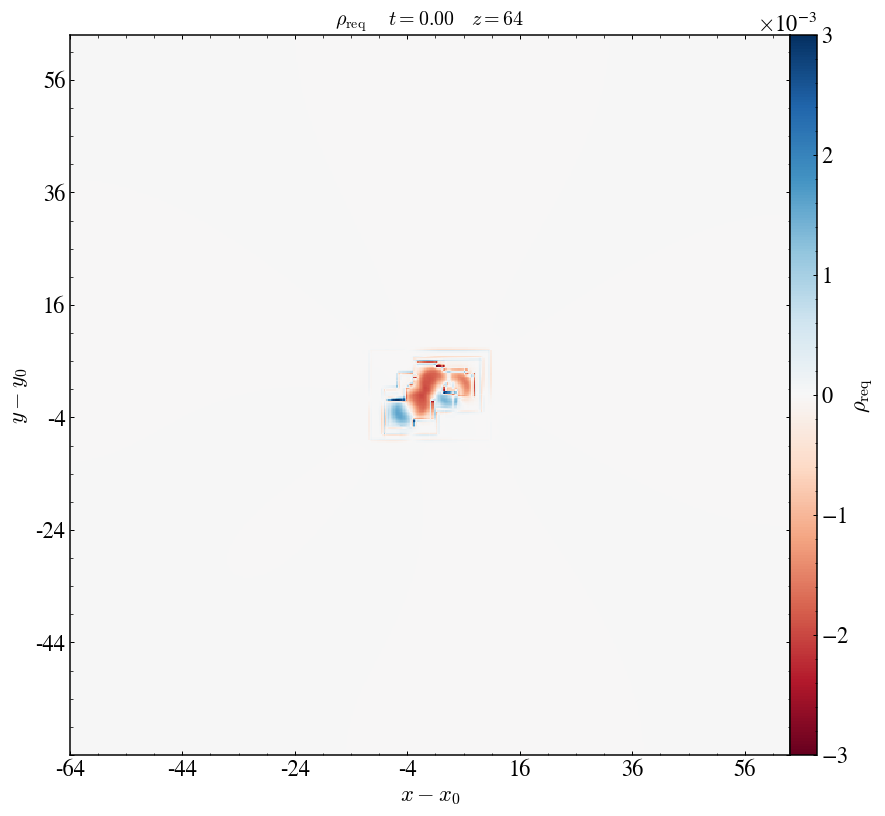
\includegraphics[width=0.245\textwidth]{fig_rf_rho_t0.png}\hfill
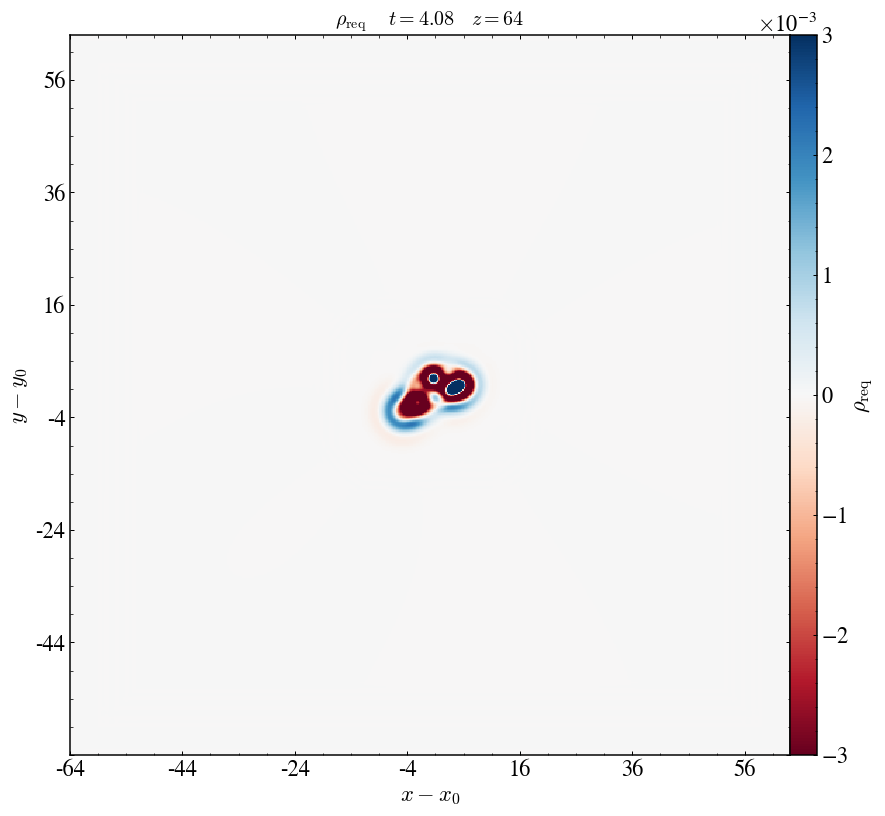
\includegraphics[width=0.245\textwidth]{fig_rf_rho_t4.png}\hfill
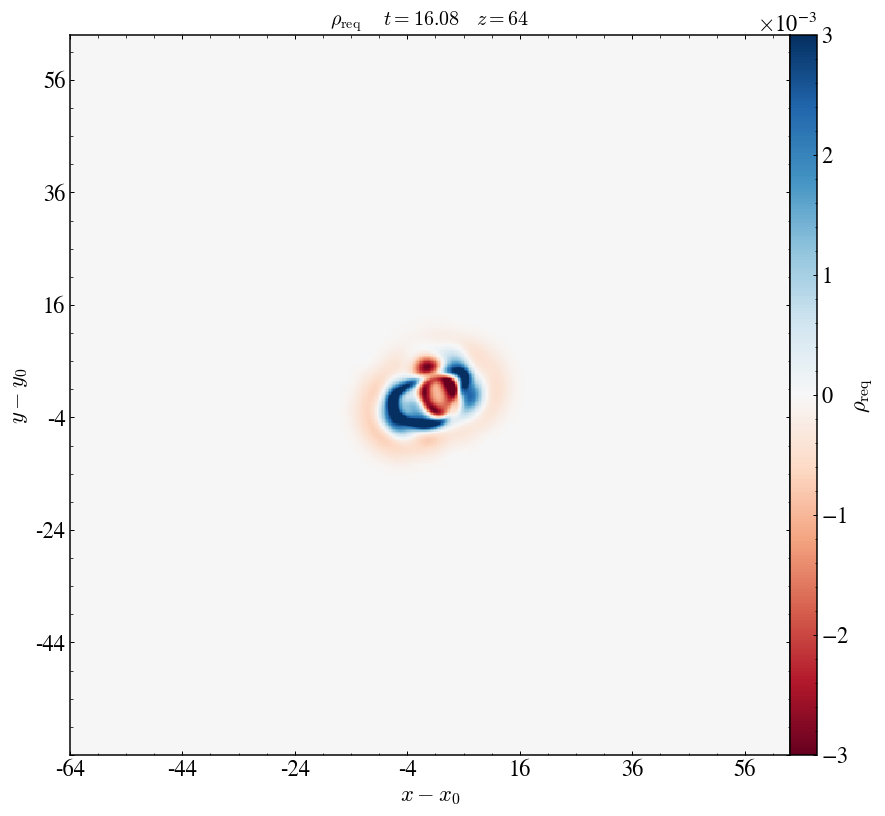
\includegraphics[width=0.245\textwidth]{fig_rf_rho_t16.png}\hfill
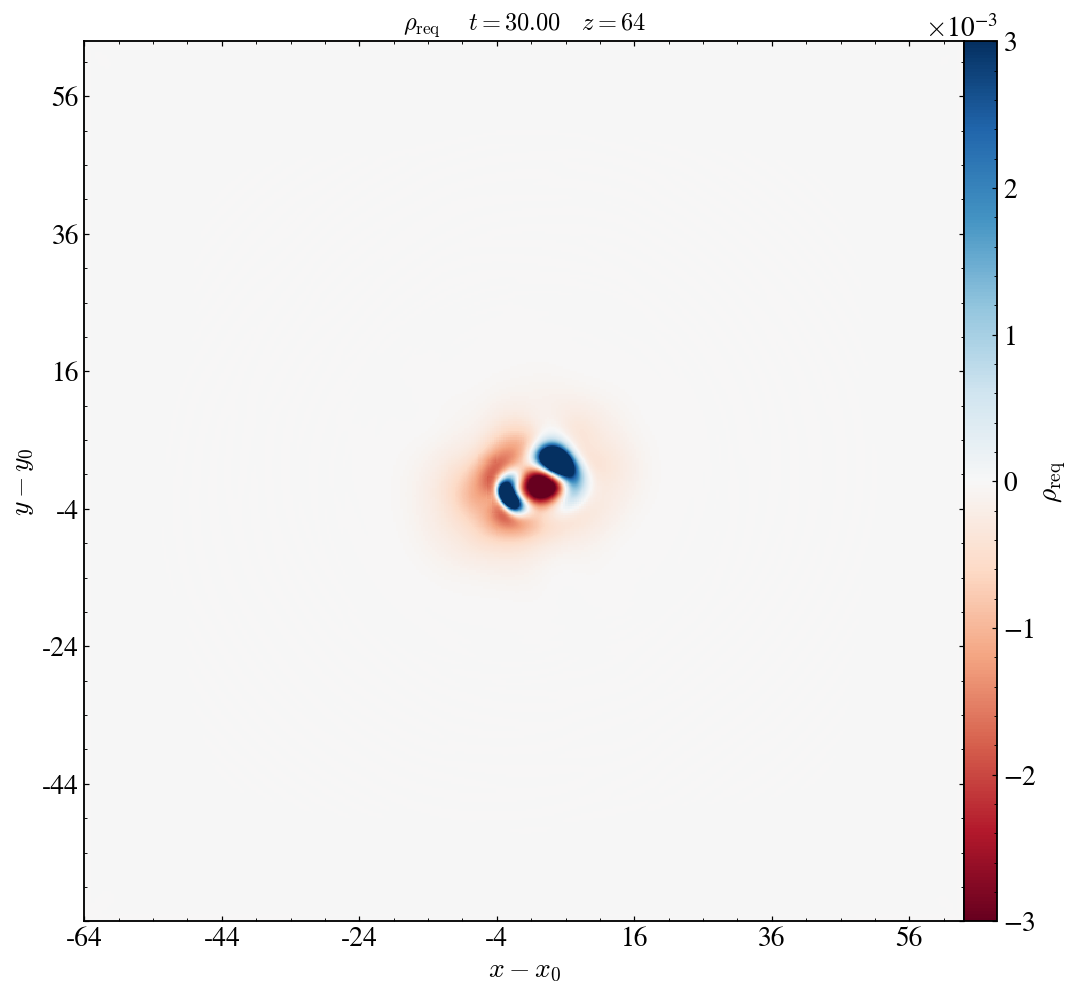
\includegraphics[width=0.245\textwidth]{fig_rf_rho_t30.png}\\[2pt]
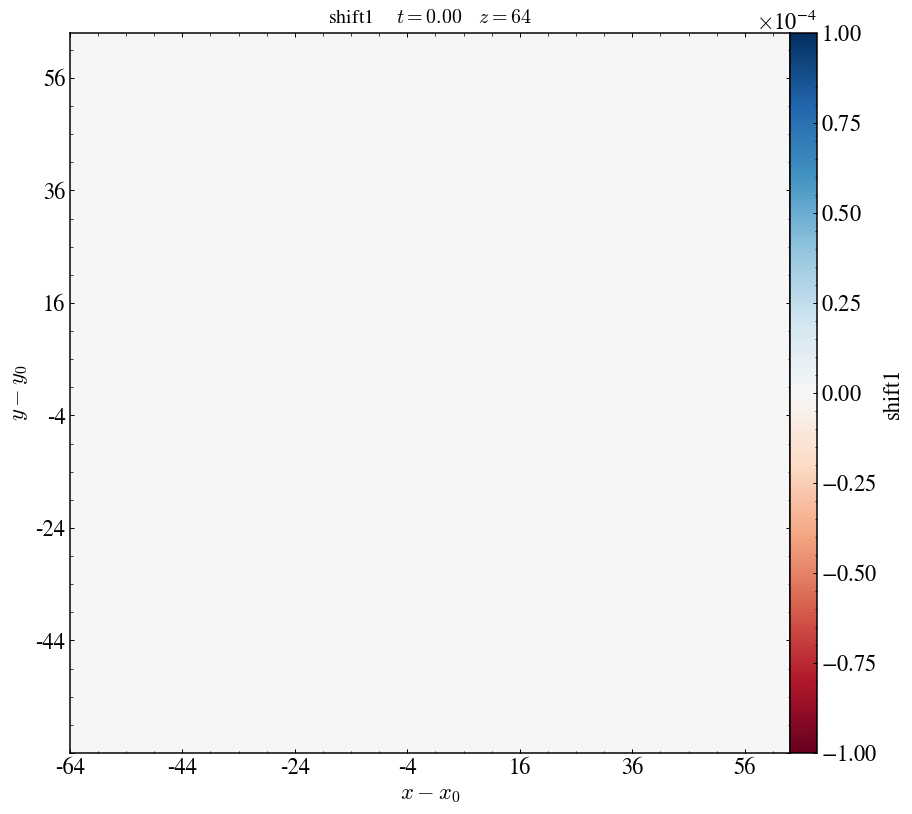
\includegraphics[width=0.245\textwidth]{fig_rf_shift_t0.png}\hfill
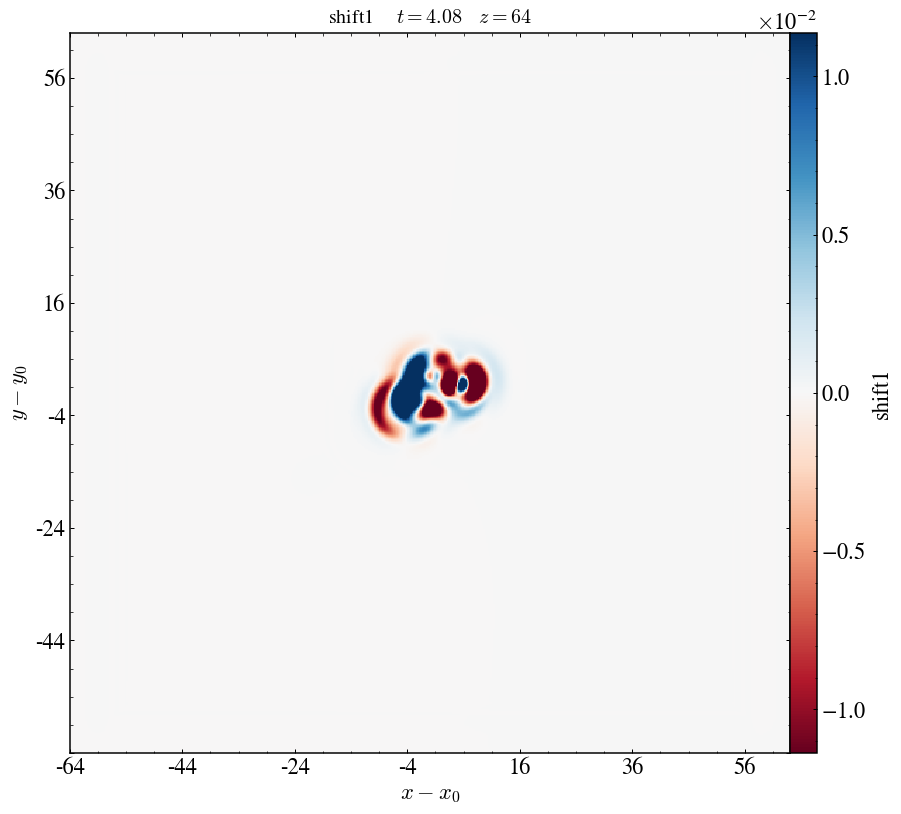
\includegraphics[width=0.245\textwidth]{fig_rf_shift_t4.png}\hfill
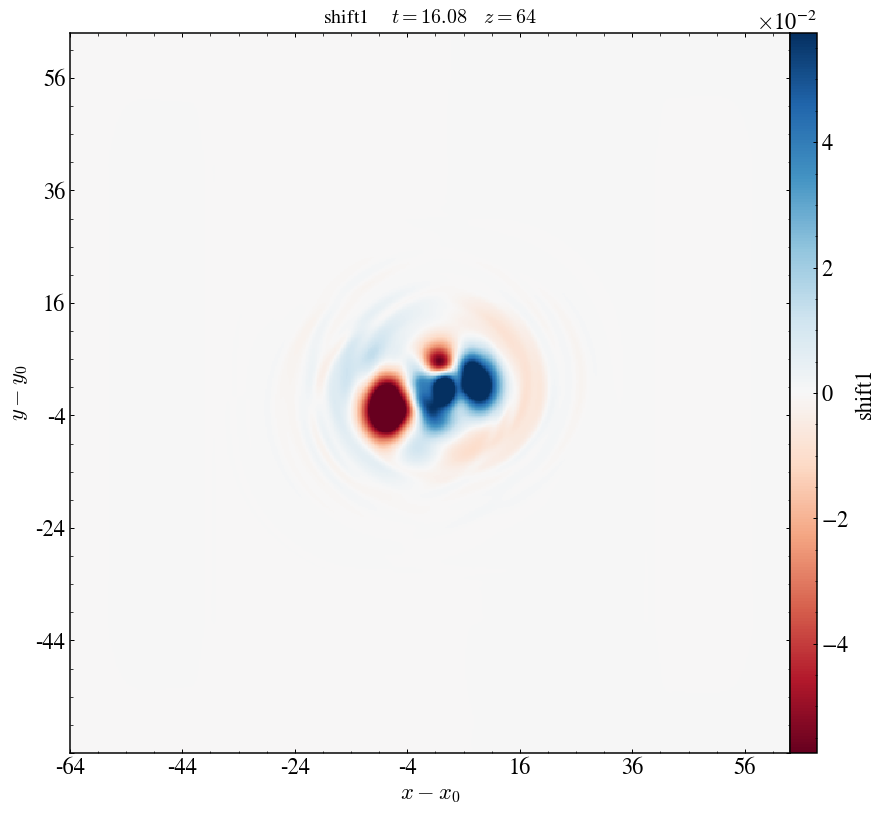
\includegraphics[width=0.245\textwidth]{fig_rf_shift_t16.png}\hfill
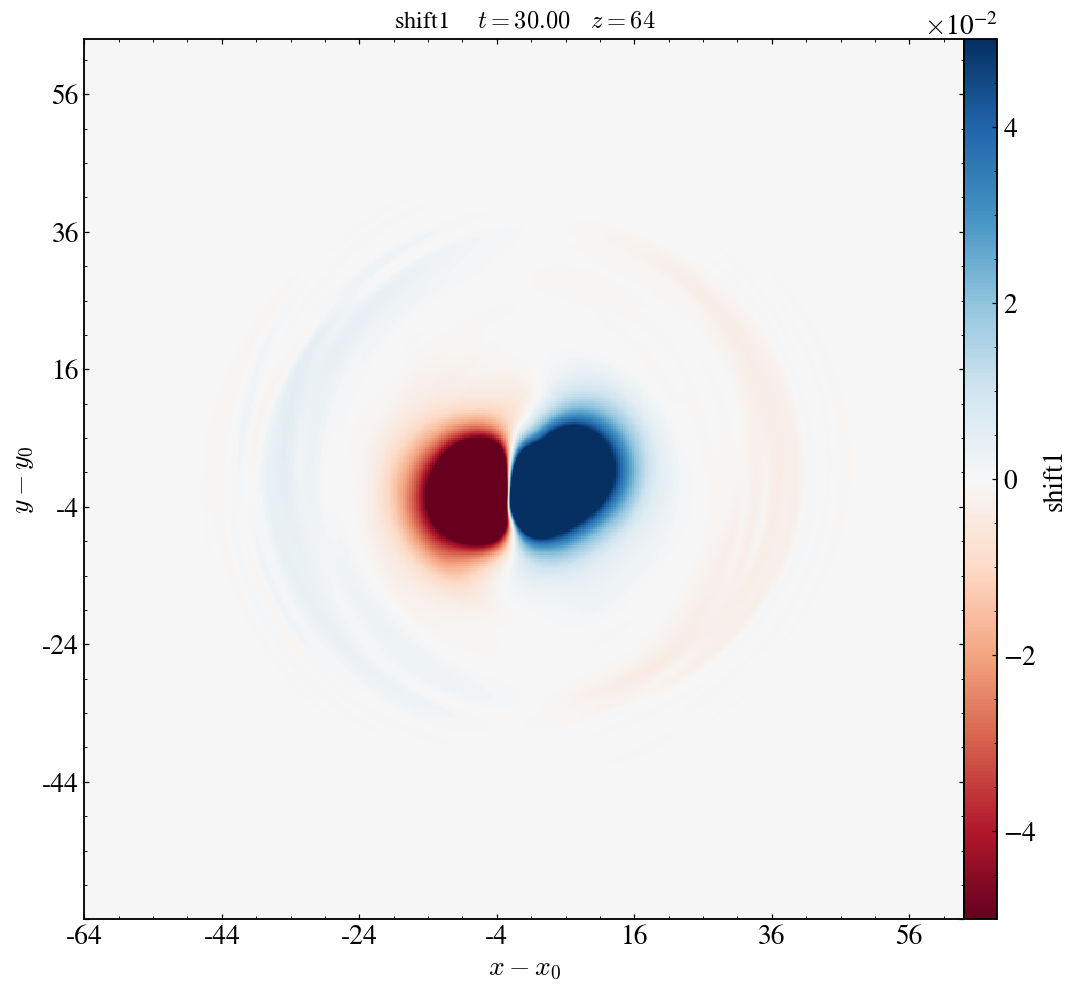
\includegraphics[width=0.245\textwidth]{fig_rf_shift_t30.png}
\caption{Evolving dynamics of candidate~146 in the finest run (RF, $N=384$),
mid-plane ($z=z_0$) slices at $t=0,4,16,30$. \emph{Top row:} required energy
density $\rho_{\rm req}$, with blue the canonical ($+\rho$) lumps and red the
phantom ($-\rho$) lumps---a direct view of the negative-energy sector of
Sec.~\ref{sec:phantom_action}. \emph{Bottom row:} the shift component
$\beta^{x}$ along the null-probe axis. Its bipolar structure is why frame
dragging does not carry the shortcut
(Table~\ref{tab:mechanism_ablation}); the transporting geometry is the
conformal well dug by the phantom lumps in the top row. The channel is
strongest just after pump-off ($t=4$, the peak-$f_{\rm geo}$ launch); by
$t=30$ both the matter and the shift structure have spread and weakened,
consistent with the transient nature of the shortcut.}
\label{fig:rf_field_maps}
\end{figure*}

\subsection{Transport mechanism: conformal contraction, not frame dragging}
\label{sec:mechanism}

The obvious candidate mechanism is frame dragging. Each Q-ball lump oscillates
with $\Pi\neq0$, so by Eq.~\eqref{eq:scalar_sources} it carries a momentum
density $S_i$ that sources a shift $\beta^i$, and a shift tilts the local light
cones---which is how the Alcubierre family transports. The shift is certainly
there: it vanishes identically on the initial slice, and the moving-puncture
gauge then grows it out of $S_i$ and $A_{ij}$ until the peak corridor value
$|\beta^{x}|$ reaches $4.3\times10^{-2}$ at the headline launch, an order of
magnitude above the endpoint values of Table~\ref{tab:endpoint_gauge}. But it
is bipolar---the corridor spans $\beta^{x}\in[-2.0,+4.3]\times10^{-2}$, the
visual signature in the bottom row of Fig.~\ref{fig:rf_field_maps}---and that
matters more than its amplitude.

To attribute the timing gain we re-trace the headline five-ray fan through the
stored metric stack with one ADM field at a time replaced by its flat value
(Table~\ref{tab:mechanism_ablation}). These are kinematic substitutions on the
stored spacetime, not new constraint solutions; they apportion the measured
$f_{\rm geo}$ rather than describe alternative universes. The result inverts the
naive expectation. Deleting the shift entirely \emph{improves} the shortcut,
$20.2\%\to22.8\%$: because $\beta^{x}$ changes sign along the corridor, the
segments that speed a $+x$ ray are more than cancelled by those that slow it,
so net frame dragging costs about $2.5$ percentage points, and a pure-shift
geometry transports no faster than Minkowski at all. The other two fields carry
the effect: flattening the lapse collapses $f_{\rm geo}$ to $1.7\%$, and the
spatial metric alone already delivers $6.8\%$.

Both surviving contributions trace to the phantom sector rather than to the
matter current. The negative-energy lumps contract the corridor, holding its
proper length below the coordinate separation $14.4$ throughout the flight
(Sec.~\ref{sec:endpoint_gauge}), and they raise the clock rate along it: the
corridor-averaged lapse, $0.955$ at launch, crosses unity at $t\approx6.5$ and
peaks at $1.34$ mid-transit. Candidate~146 is therefore a \emph{conformal-well
precursor}: the exotic matter digs a shortened, fast-clock corridor, and the
shift it inevitably also sources is a mild parasitic drag.

This also settles what would otherwise be a loose end. The spatial-metric-only
entry, $6.8\%$ (RM) and $7.0\%$ (RC), lands at the lower edge of the freely
falling observer band $f_{\rm ff}=7.0$--$7.7\%$ measured independently in
Sec.~\ref{sec:freefall_metric}, because the free-fall receiver reports the
proper-distance contraction and discards the slicing-dependent lapse
elevation---exactly the ${\sim}13$-point remainder of the coordinate figure.
So $20.2\%$ is the coordinate-referenced advantage in the selected gauge,
$7.6\%$ is the observer-level one, and the ablation says which piece of
geometry supplies each.

\begin{table}[tbp]
\caption{Mechanism ablation for candidate~146: peak evolving $f_{\rm geo}$
when one ADM field of the stored metric stack is replaced by its flat value,
with the same five-ray fan and launch $t_{\rm emit}=4$. Substitutions are
diagnostic, not constraint-satisfying. Removing the shift \emph{raises} the
shortcut; removing the lapse elevation removes almost all of it. Baseline
re-traces of the archived stacks give $20.15\%$ (RM) and $20.60\%$ (RC),
within $0.2$ percentage points of Table~\ref{tab:matrix}.
Source: \texttt{mechanism\_ablation.txt}.}
\label{tab:mechanism_ablation}
\begin{ruledtabular}
\begin{tabular}{lcc}
metric retained & $f_{\rm geo}$ (RM) & $f_{\rm geo}$ (RC) \\
\hline
all (baseline)                                   & $20.15\%$ & $20.60\%$ \\
$\beta^i\to0$ (no frame dragging)                & $22.76\%$ & $23.10\%$ \\
$\alpha\to1$ (no lapse elevation)                & $1.70\%$  & $1.63\%$  \\
$\gamma_{ij}$ only ($\alpha=1$, $\beta^i=0$)     & $6.83\%$  & $6.96\%$  \\
$\beta^i$ only ($\alpha=1$, $\gamma_{ij}=\delta_{ij}$) & $0.00\%$ & $0.00\%$ \\
\end{tabular}
\end{ruledtabular}
\end{table}

\subsection{4D falsification certificate}

The headline claim is operational: in the RM run, null rays between the fixed
endpoints arrive earlier than in flat space. Table~\ref{tab:certificate}
lists the quantities reported by the evolving-geodesic probe.

\begin{table}[tbp]
\caption{Evolving null-geodesic transport certificate for candidate~146 in
the headline RM run ($L=128$, $N=256$, $t=30$).}
\label{tab:certificate}
\begin{ruledtabular}
\begin{tabular}{ll}
quantity & value \\
\hline
peak 4D $f_{\rm geo}$ & $20.21\%$ \\
frozen-peak $f_{\rm geo}$ & $29.45\%$ \\
rays reached & $5/5$ \\
$t_{\rm emit}$ & $4.00$ \\
$t_{\rm arrival}$ & $15.49$ \\
$t_{\rm min}=t_{\rm arrival}-t_{\rm emit}$ & $11.49$ \\
$t_{\rm transit}^{\rm flat}$ & $14.40$ \\
$h_{\rm quality\_ok}$ & true
($h_{\rm rel}^{\rm max}=2.19\times10^{-3}$) \\
search-tier peak (CMA-ES) & $20.12\%$ ($3/3$ rays) \\
\end{tabular}
\end{ruledtabular}
\end{table}

Explicitly,
$(t_{\rm flat}-t_{\rm min})/t_{\rm flat}
=(14.40-11.49)/14.40=20.21\%$, matching
Eq.~\eqref{eq:f_geo}. The endpoint timing corresponds to an effective
$c/(1-f_{\rm geo})\simeq1.25c$ relative to the matched flat path; nothing
physical moves outside its local light cone
(Fig.~\ref{fig:timing_protocols}a).

The frozen peak in the same table reaches $29.45\%$, some nine percentage
points higher, and the gap is physical rather than an error bar: the frozen
trace assumes one snapshot persists for the whole flight, whereas the 4D trace
watches the channel open and then weaken while the photon is inside it. Only
the latter certifies transport. The frozen peak is itself stable across the
resolution ladder ($29.1$--$29.5\%$), so the gap is not a snapshot-quality
artifact. Sweeping the launch time (Fig.~\ref{fig:fgeo_validation}) shows the
evolving advantage peaking at $t_{\rm emit}=4$ in all three runs and decaying
monotonically thereafter, so successful transport coexists with the dispersal
of Sec.~\ref{sec:dispersion} only inside a finite window.

\begin{figure}[tbp]
\centering
\begin{tikzpicture}
\begin{axis}[
  width=0.94\columnwidth,height=0.58\columnwidth,
  grid=major,grid style={gray!20},
  tick label style={font=\small},label style={font=\small},
  legend style={
    at={(0.5,1.04)},anchor=south,
    font=\scriptsize,draw=none
  },
  xlabel={$t_{\rm emit}$},ylabel={$f_{\rm geo}$ [\%]},
  xmin=0,xmax=12,ymin=0,ymax=22,
  legend columns=3
]
\addplot[blue,mark=*] table[x=t,y=RC]{data/fgeo_sweeps.txt};
\addlegendentry{RC ($N{=}192$)}
\addplot[black,thick,mark=square*] table[x=t,y=RM]{data/fgeo_sweeps.txt};
\addlegendentry{RM ($N{=}256$)}
\addplot[red,mark=triangle*] table[x=t,y=RF]{data/fgeo_sweeps.txt};
\addlegendentry{RF ($N{=}384$)}
\end{axis}
\end{tikzpicture}
\caption{Evolving null-geodesic emission sweeps
($t_{\rm emit}=0,2,\ldots,12$) for all three resolution-matrix runs; the
metric evolves to $t=30$, but late launches lack enough remaining geometry
for a complete transit. All runs peak at $t_{\rm emit}=4$, just after PD
pump-off, and agree within $0.26$ percentage points. Every launch has
$5/5$ rays reaching and passes the null-Hamiltonian quality gate; at
$t_{\rm emit}=12$ the rays arrive no earlier than the flat baseline, so the
clamped advantage [Eq.~\eqref{eq:f_geo}] is zero.}
\label{fig:fgeo_validation}
\end{figure}

\subsection{Endpoint gauge and proper-time invariance}
\label{sec:endpoint_gauge}

The timing advantage of Eq.~\eqref{eq:f_geo} compares two \emph{coordinate}
transit durations between fixed endpoints, which is only a physical statement
if those endpoints behave as nearly stationary, nearly flat observers---a deep
lapse well ($\alpha\ll1$) there could manufacture a coordinate advance with no
proper-time content. The emitter and receiver sit on the propagation axis at
$A=(56.8,64,64)$ and $B=(71.2,64,64)$ in the $L=128$ box centered on
$(64,64,64)$, a corridor of coordinate length $t_{\rm flat}=14.4$. At the
headline launch $t_{\rm emit}=4$ both are close to flat and stationary
(Table~\ref{tab:endpoint_gauge}): $\alpha_A=0.96$, $\alpha_B=0.99$, and
$|\beta^i|\lesssim3.5\times10^{-2}$. The lapse never enters the dangerous
$\alpha\ll1$ regime; at late times it drifts modestly \emph{above} unity
($\alpha\lesssim1.2$), which if anything makes the coordinate advantage
conservative, since a stationary clock with $\alpha>1$ accumulates proper time
faster than coordinate time.

\begin{table}[tbp]
\caption{Lapse $\alpha$ and shift magnitude $|\beta^i|$ at the fixed probe
endpoints $A$ (emitter) and $B$ (receiver) in RM, sampled through the emission
window. The endpoints remain near-stationary ($|\beta^i|\ll1$) and out of any
deep-lapse well ($\alpha\ge0.95$ at launch).
Source: \texttt{endpoint\_gauge\_rm.txt}.}
\label{tab:endpoint_gauge}
\begin{ruledtabular}
\begin{tabular}{rcccc}
$t$ & $\alpha_A$ & $|\beta^i|_A$ & $\alpha_B$ & $|\beta^i|_B$ \\
\hline
 0 & $1.000$ & $0$                  & $1.000$ & $0$ \\
 4 & $0.960$ & $4.5\times10^{-3}$   & $0.993$ & $3.5\times10^{-2}$ \\
 8 & $0.946$ & $1.7\times10^{-2}$   & $1.048$ & $9.3\times10^{-2}$ \\
12 & $1.179$ & $1.2\times10^{-2}$   & $1.209$ & $1.3\times10^{-2}$ \\
15 & $1.172$ & $6.9\times10^{-2}$   & $1.118$ & $7.1\times10^{-2}$ \\
\end{tabular}
\end{ruledtabular}
\end{table}

As a gauge-robustness check, we re-express the advantage in the proper time of
a static receiver at $B$, whose clock ticks at $d\tau=\sqrt{-g_{00}(B)}\,dt$.
Integrating the measured $g_{00}(B,t)$ from $t_{\rm emit}$ to each arrival, the
curved signal reaches $B$ at $\tau_{\rm curved}=12.61$ and the matched
flat-rate signal at $\tau_{\rm flat}=15.66$, giving
\begin{equation}
f_{\rm geo}^{\tau}=\frac{\tau_{\rm flat}-\tau_{\rm curved}}{\tau_{\rm flat}}
=19.5\%,
\label{eq:proper_time_fgeo}
\end{equation}
within $0.7$ percentage points of the coordinate value $20.2\%$. The advantage
is therefore robust against lapse/shift coordinate effects in the selected
gauge: it survives conversion to the physical clock of a stationary receiver
at~$B$. This does not constitute a gauge-invariant proof---the receiver is
defined by fixed coordinates, not a geometrically selected worldline---but
it confirms the signal is not a coordinate artifact of the $1+\log$ slicing.

A complementary check concerns proper \emph{distance}. The negative-energy
sources contract the spatial metric along the corridor, so the coordinate
separation $14.4$ overstates the proper length of the $A$--$B$ line:
integrating $\int\sqrt{\gamma_{xx}}\,dx$ in the stored RM metric stack gives
$13.85$ at $t=0$, $13.60$ at the stored slice nearest the headline launch
($t=4.32$), and a value inside $[13.08,13.67]$ throughout the flight window.
Part of the coordinate advantage is therefore genuine spatial contraction
sourced by the exotic matter---a physical effect, and one the ablation of
Sec.~\ref{sec:mechanism} isolates quantitatively. Even under the most
conservative renormalization, comparing the curved transit $t_{\rm min}=11.49$
against a flat transit across the \emph{smallest} instantaneous proper length,
$(13.08-11.49)/13.08=12.2\%$, the advantage stays strictly positive. We
quote the coordinate-referenced $20.2\%$ as the headline number because
Eq.~\eqref{eq:f_geo} defines its flat baseline by the fixed coordinate
endpoints, but both normalizations certify an early arrival.

\subsection{Resolution and domain matrix}

Validation comprises two complementary tests of candidate~146
(Table~\ref{tab:matrix}). At fixed domain $L=128$, a resolution
ladder---RC ($N=192$), RM ($N=256$), RF ($N=384$)---probes continuum
stability. At fixed spacing $h=0.500$, a domain ladder---DS ($L=96$) and DL
($L=160$)---probes sensitivity to outer-boundary placement, all evolutions
carrying non-periodic Sommerfeld (radiative) conditions on all six faces. RM
is the reference configuration quoted elsewhere in this paper.

\begin{table}[tbp]
\caption{Resolution and domain matrix for candidate~146. Every run uses
three refinement levels above the base grid (\texttt{max\_level}$=3$,
\texttt{regrid\_threshold}$=0.02$) and terminates at $t=30$. Peak
$f_{\rm geo}$ is the maximum evolving 4D null-geodesic timing advantage;
frozen peak is the maximum of the frozen-slice $f_{\rm geo}$ time series;
$f_{\rm ff}$ is the freely falling observer metric
(Sec.~\ref{sec:freefall_metric}), taken from three matched companion
integrations (\texttt{bcma\_*\_freefall\_corrected\_*}) whose metric stacks are
bit-identical to the runs in the other columns.}
\label{tab:matrix}
\begin{ruledtabular}
\begin{tabular}{lrrrrrrr}
run & $L$ & $N$ & $h$ & peak $f_{\rm geo}$ & frozen peak & $f_{\rm ff}$ & $t_{\rm emit}$ \\
\hline
RC & 128 & 192 & 0.667 & 20.44\% & 29.15\% & 7.69\% & 4 \\
RM & 128 & 256 & 0.500 & 20.21\% & 29.45\% & 7.62\% & 4 \\
RF & 128 & 384 & 0.333 & 20.19\% & 29.54\% & 7.01\% & 4 \\
DS & 96 & 192 & 0.500 & 20.19\% & 29.21\% & --- & 4 \\
DL & 160 & 320 & 0.500 & 20.22\% & 29.44\% & --- & 4 \\
\end{tabular}
\end{ruledtabular}
\end{table}

On the resolution ladder the evolving timing advantage runs
$20.44\%\to20.21\%\to20.19\%$: monotonically decreasing, with a fine--medium
relative difference of $0.13\%$, far inside the $10\%$ acceptance tolerance
fixed before the ladder was run. The frozen peak stays at $29.1$--$29.5\%$ and
the freely falling observer metric at $7.01$--$7.69\%$, the latter's $8\%$
fine--medium spread indicating mild but acceptable resolution dependence in the
proper-time measurement. On the domain ladder, DS and DL differ from RM by at
most $0.12\%$ relative, with five of five rays reaching in every run.
Outer-boundary reflections therefore do not set the reported advantage on
$t\le30$, consistent with a causal estimate for the $L=128$ box: in
$1{+}\log$ slicing, gauge modes travelling at ${\sim}\sqrt{2}\,c$ need
$t\gtrsim L/(2\sqrt{2})\approx45$ to reach the central region.

For unequal spacings, a Richardson estimate assumes
\begin{equation}
 Q(h)=Q_0+Ch^p,\qquad
 \frac{Q_c-Q_m}{Q_m-Q_f}
 =\frac{h_c^p-h_m^p}{h_m^p-h_f^p}.
 \label{eq:richardson_order}
\end{equation}
Applied to the $f_{\rm geo}$ triplet at the actual spacings
$(h_c,h_m,h_f)=(0.667,0.500,0.333)$, Eq.~\eqref{eq:richardson_order} returns an
unstable exponent ($p\approx8.7$) fixed by a fine--medium difference of one
significant figure: the sequence is consistent with rapid convergence but
cannot pin down $p$. The anomaly is expected here, because $f_{\rm geo}$ is not
a pointwise field value but an arrival-time functional---root-found from a
detector crossing along five rays integrated through a stack stored at finite
cadence on a moving refinement hierarchy, then reported as the best member of
the fan over a discrete $t_{\rm emit}$ sweep. Regridding times, stack
interpolation, and a different ray or emission time winning at a different
resolution all make the dependence non-smooth rather than $Ch^p$, and once the
smooth truncation error has fallen to the $10^{-3}$ level seen here they
dominate the increments the estimator is built from. We therefore measure the
observed order on the constraint norms instead
(Fig.~\ref{fig:constraints}a): over the ignition window $1.5\le t\le5$ the
Hamiltonian residual converges at median order $p_{\mathcal H}\approx3.3$ and
the momentum residual at $p_{\mathcal M}\approx2.8$, consistent with the
high-order finite-difference scheme. We accept the $20.2\%$ shortcut as
continuum-stable without quoting a formal extrapolated value.

\begin{figure}[tbp]
\centering
\begin{tikzpicture}
\begin{semilogyaxis}[
  width=0.97\columnwidth,height=0.55\columnwidth,
  xlabel={$t$},ylabel={$\|\mathcal H\|_{L^2}$},
  xmin=0,xmax=30,ymin=5e-4,ymax=8e-3,
  grid=major,grid style={gray!20},
  legend style={font=\scriptsize,draw=none,at={(0.98,0.05)},anchor=south east},
  title={\small (a) Resolution convergence}
]
\addplot[blue,thin] table[x=t,y=ham_RC]{data/constraints_resolution.txt};
\addlegendentry{RC ($N{=}192$)}
\addplot[black,thick] table[x=t,y=ham_RM]{data/constraints_resolution.txt};
\addlegendentry{RM ($N{=}256$)}
\addplot[red,dashed,thick] table[x=t,y=ham_RF]{data/constraints_resolution.txt};
\addlegendentry{RF ($N{=}384$)}
\end{semilogyaxis}
\end{tikzpicture}

\vspace{0.4cm}

\begin{tikzpicture}
\begin{semilogyaxis}[
  width=0.97\columnwidth,height=0.55\columnwidth,
  xlabel={$t$},ylabel={$\|\mathcal C\|_{L^2}$},
  xmin=0,xmax=30,ymin=2e-5,ymax=8e-3,
  grid=major,grid style={gray!20},
  legend style={font=\small,draw=none,at={(0.98,0.05)},anchor=south east},
  title={\small (b) RM constraint norms}
]
\addplot[black,thick] table[x=t,y=ham]{data/constraints_rm.txt};
\addlegendentry{$\|\mathcal H\|_2$}
\addplot[red,dashed,thick] table[x=t,y=mom]{data/constraints_rm.txt};
\addlegendentry{$\|\mathcal M\|_2$}
\end{semilogyaxis}
\end{tikzpicture}
\caption{Constraint diagnostics.
(a)~Hamiltonian constraint norm across the Richardson ladder;
the three resolutions overlie closely with observed order
$p_{\mathcal H}\approx3.3$ (median) in the ignition window.
(b)~Constraint norms in the headline RM run; the complete $3000$-step
diagnostic is plotted from a decimated table; maxima are evaluated from
the full data.}
\label{fig:constraints}
\end{figure}

\subsection{Evolution constraints}

For RM, the volume-weighted norms remain below
$\|\mathcal H\|_2=4.73\times10^{-3}$ and
$\|\mathcal M\|_2=9.16\times10^{-4}$ through $t=30$
(Fig.~\ref{fig:constraints}b). These are comparable to the search-tier values
and remain bounded throughout the evolution. The constraint norms peak during
the early driven phase ($t\lesssim4$) and then plateau or slowly grow during
the free evolution, consistent with the dispersing matter producing less
active refinement at late times.

\subsection{Evolution with the PD controller disabled}
\label{sec:pump_free}

Because the PD trajectory controller (Sec.~\ref{sec:pd_pump}) is an
external, non-Lagrangian source, we repeat the HQ evolution of
candidate~146 with the controller disabled from $t=0$
($t_{\rm pump}=0$), holding all other settings fixed ($L=128$, $N=256$,
three refinement levels, $t=30$). Table~\ref{tab:pump_compare} compares this
pump-free integration (PF-RM) with the default pump-on twin (RM;
$t_{\rm pump}=4$).

\begin{table}[tbp]
\caption{Matched HQ comparison of candidate~146 with the PD controller on
through $t=4$ (RM) and disabled from $t=0$ (PF-RM). Both runs use
$L=128$, $N=256$, and $t=30$. Evolving $f_{\rm geo}$ is the 4D
null-geodesic timing advantage; $E_{\rm pump}$ is the integrated pump work
recorded in \texttt{collapse\_diagnostics.dat}; $S$ is the final
\texttt{general\_ftl} score.}
\label{tab:pump_compare}
\begin{ruledtabular}
\begin{tabular}{lcc}
metric & RM ($t_{\rm pump}=4$) & PF-RM ($t_{\rm pump}=0$) \\
\hline
evolving $f_{\rm geo}$ & $20.21\%$ & $20.46\%$ \\
rays / $h$ quality & $5/5$, pass & $5/5$, pass \\
best $t_{\rm emit}$ & $4$ & $12$ \\
$E_{\rm pump}$ & $1.6\times10^{-17}$ & $0$ \\
confined ($t{=}0\to30$) & $72\%\to11\%$ & $72\%\to2\%$ \\
rms spread ratio & $3.27$ & $3.07$ \\
final score $S$ & $126.3$ & $47.0$ \\
\end{tabular}
\end{ruledtabular}
\end{table}

With the PD term off, the evolving timing advantage remains
$f_{\rm geo}=20.46\%$---within $1.2\%$ relative of the pump-on value---with
all five rays reaching and the null-Hamiltonian quality gate satisfied. The
integrated pump work vanishes identically, so the advantage cannot be
ascribed to external PD energy injection. The channel does open more slowly:
the emission optimum shifts from $t_{\rm emit}=4$ to $t_{\rm emit}=12$ and
migrates from the $x$ axis to the $z$ axis of the probe, while the peak
amplitude is essentially unchanged. Because $t_{\rm emit}=12$ is the last
point of the emission sweep, the pump-free value is strictly a lower bound on
that run's peak advantage; the channel may still be opening when the sweep
window closes.

The controller's principal effect is therefore on matter retention, not on
$f_{\rm geo}$: at $t=30$ the pump-on run still confines ${\sim}11\%$ of the
matter against ${\sim}2\%$ without it. That is also why the composite score
falls from $S=126.3$ to $S=47.0$---confinement-gated terms penalize the faster
dispersal, while the timing advantage itself is unchanged. In both
integrations the shortcut remains a transient precursor coexisting with
dispersing exotic matter.

We nonetheless keep RM, not PF-RM, as the headline configuration. The first
reason is consistency with the search: the entire MAP-Elites and CMA-ES
campaign ran with the controller enabled through $t_{\rm pump}=4$, so
candidate~146 is an elite \emph{of that protocol}. PF-RM re-evaluates the same
genome under a different one; it is a control, not an independently optimized
solution, and its emission optimum has already migrated to the last point of
the sweep window. The second reason is the five-fold confinement difference
above. Structural persistence is what distinguishes a precursor from a burst of
dispersing scalar field, and it is the property the controller buys. Read as
engineering rather than as a Lagrangian, the PD term is a placeholder for the
station-keeping actuation any real device would require, and the configuration
worth reporting is the one under active control. Nothing in the transport
certificate turns on the choice: the headline ray launches after the controller
is off, and the two protocols agree on $f_{\rm geo}$ to within $1.2\%$
relative. PF-RM's role is to establish that the control is not manufacturing
the geometry.


\section{Discussion}
\label{sec:discussion}

\subsection{The dispersion problem}
\label{sec:dispersion}

Candidate~146 should be read against the many configurations that did not work.
Across roughly a dozen ansatz families and several full MAP-Elites campaigns we
repeatedly found the same failure mode: the supporting matter disperses and the
transport channel closes with it. Spherical-harmonic shells yielded a single
weak hit in ${\sim}\!200$ evaluations. Free massive scalar packets have no bound
state and blow apart almost immediately. Bicomplex phantom lumps \emph{without}
Q-ball self-binding (an earlier, pre-soliton family) opened a
gauge-invariant shortcut but lost ${\sim}\!98\%$ of their structure by $t=16$.
Boosted and stiffened Q-ball variants improved early confinement but still
sheared apart once placed on an orbit. CMA-ES bought back some persistence
(Sec.~\ref{sec:strength_vs_persistence}), but candidate~146 still ends the
production window at ${\sim}11\%$ confinement.

Beyond dispersal, the HQ runs develop a corroborated trapped surface at late
times ($t\approx27$ in the resolution ladder, $t\approx24$ in the pump-free
twin), with a minimum expansion scalar $\theta_+\approx-0.9$ and
$r_{\rm AH}\approx10.8$ code units. The headline geodesic launches at
$t_{\rm emit}=4$ and arrives at $t\approx15.5$, well before any apparent
horizon forms, so the transport certificate is unaffected. The collapse is
itself a symptom of transience: once the exotic matter disperses, the residual
positive-energy content exceeds the threshold for gravitational collapse. A
transient shortcut is reproducible and robust here; a long-lived, well-confined
channel remains an open problem.

\subsection{Canonical-only (positive-energy) search bound}
\label{sec:canonical_bound}

Reported positive-energy warp solitons~\cite{lentz21,fell21} and their
critique~\cite{santiago2022} make the positive-energy sector the natural
next target for an automated search. To test whether the same five-lump
bicomplex Q-ball genome can produce a
gauge-invariant timing advantage without phantom sources, we reran the
MAP-Elites campaign of Sec.~\ref{sec:methodology} with every per-lump
exotic amplitude pinned to zero, retaining the canonical Klein--Gordon
sector, retrograde-orbit bias, and post-load constraint gates. Over
$200$ evaluations ($105$ GPU-accepted; $95$ rejected at the post-load
Hamiltonian $L^2$ gate), the archive champion reached only
$S\approx47.4$ (eval.~130), and the evolving geodesic fraction
satisfied
\begin{equation}
  \max_{\theta\in\mathcal{A}_{\rm can}}
  f_{\rm geo}^{\rm evol}(\theta)
  = 0
  \qquad
  (N_{\mathrm{ok}}=105).
  \label{eq:canonical_bound}
\end{equation}
Several accepted genomes developed superluminal local coordinate signal
speeds ($\max v_{\rm loc}>1$, a gauge-dependent diagnostic) or early
apparent horizons, but none completed a
null-timing advantage under the evolving-geodesic certificate. Within this
ansatz and search budget, a completed $f_{\rm geo}>0$ therefore appears to
require the phantom sector used by candidate~146; the positive-energy
search remains open for broader matter families and longer $t_{\rm stop}$.

\subsection{Limitations of the matter-first approach}
\label{sec:limitations}

The matter-first approach (Sec.~\ref{sec:intro}) is complementary to
geometry-first~\cite{helmerich2024warpfactory}: every candidate is
constraint-satisfying by construction, but the search is confined to the
chosen matter model. Three specific limitations follow.
\begin{enumerate}
  \item \textbf{Ansatz dependence.} The pipeline discovers only what the
    parameterized matter family can express. The 39-dimensional bicomplex
    Q-ball genome covers orbital arrangements of five solitons but cannot
    represent, e.g., anisotropic fluids, higher-spin fields, or engineered
    equation-of-state shells. Broadening the matter sector is the most direct
    route to new mechanism families.
  \item \textbf{$\mathbb{R}^3$ spatial topology.} Both the constraint solve
    and the Cauchy evolution operate on a topologically trivial slice
    ($\mathbb{R}^3$ with Sommerfeld radiative boundaries). Features that exist
    only in the full four-dimensional manifold---wormhole throats, handles,
    other nontrivial $\mathbb{R}^4$ structures---cannot be represented on the
    initial slice and are invisible to the search. Reaching them would need an
    extended initial-data formalism (puncture or excision methods) or a
    geometry-first seed that is subsequently evolved.
  \item \textbf{Ignition-phase controller.} The PD pump
    (Sec.~\ref{sec:pd_pump}) is a non-Lagrangian external source; results
    without it (Sec.~\ref{sec:pump_free}) are comparable. A fully
    self-consistent confinement mechanism would remove the need for any
    external drive.
\end{enumerate}

\subsection{Geometry-first kinematic ceiling}
\label{sec:geometry_ceiling}

The canonical-only bound of Sec.~\ref{sec:canonical_bound} asks how far the
search reaches within one matter model. A complementary question is purely
kinematic: setting sourceability aside, how large a frozen-slice shortcut is
available to \emph{any} asymptotically flat stationary metric of this scale?
To answer it we ran a deliberately geometry-first companion search---the very
regime the Introduction rejects for dynamics---in order to price what the
matter-first pipeline leaves on the table.

Here a stationary metric is painted directly from a genome: compact-support
radial-basis deformations of the lapse, shift, and symmetric log-spatial-metric
$S$ (with $\gamma=\exp S$ guaranteeing positive-definiteness and asymptotic
flatness), plus an analytic tail of coherent topologies---an Alcubierre shift
tube, an anisotropic ``compression tunnel,'' a conformal ``lens'' well, and a
Morris--Thorne--flavored ``throat.'' No initial-value problem is solved: the
implied stress-energy is read off as $T_{\mu\nu}=G_{\mu\nu}/8\pi$, and only the
\emph{frozen} single-slice $f_{\rm geo}$ is scored, so these numbers are
\emph{not} comparable to Table~\ref{tab:certificate}.
MAP-Elites~\cite{mouret15} tiles the archive by morphology (shift fraction
$f_{\rm shift}$, running from $0$ for pure spatial curvature to $1$ for a pure
shift tube) against exotic cost $E_-=-\!\int_{\rho<0}\rho\,dV$. Three
warm-started campaigns totaling ${\sim}2000$ evaluations populate it, the last
hard-rejecting $E_->0.1$. Two settings are screening-tier rather than
continuum: the coherent analytic topologies had to be added because free-form
Gaussian bumps collapse into a maximal-shift monoculture, and the frozen probe
reads correctly only with endpoints localized about the genome support
(${\sim}8$ percentage points against diluted full-box endpoints) and $h\le0.5$
(at $h=2$ the shift wall is unresolved and under-reads by nearly a factor
of five).

Two features of the atlas (Table~\ref{tab:geometry_ceiling}) bear on the
matter-first result. First, strength is monopolized by the shift channel: the
frozen ceiling reaches $48.5\%$ for near-pure shift tubes
($f_{\rm shift}\approx0.99$), and of the $781$ accepted geometries with
$f_{\rm geo}>10\%$, $67\%$ sit at $f_{\rm shift}\ge0.5$ against only $4.5\%$ at
$f_{\rm shift}\le0.05$. Zero-shift curvature topologies do open genuine
shortcuts---the best curvature-dominated elite reaches $21.8\%$---but they are
systematically weaker. Second, none of these shortcuts is cheap: every geometry
with a positive frozen shortcut carries substantial negative energy
($E_-\sim3$--$7$), and hard-rejecting $E_->0.1$ leaves a best admissible
shortcut of $6.8\%$, a factor ${\sim}7$ below the unconstrained ceiling.
Shift-tilted and curvature-contracted shortcuts alike demand NEC violation, in
line with the classical theorems cited in Sec.~\ref{sec:intro}.

\begin{table}[tbp]
\caption{Frozen geometry-first kinematic ceiling from the stationary
MAP-Elites atlas (grid $N=64$, $L=32$; localized null-geodesic probe; no
evolution). $f_{\rm shift}$ is the morphology descriptor and
$E_-=-\int_{\rho<0}\rho\,dV$ the exotic cost. Frozen $f_{\rm geo}$ is
geometry-first and \emph{not} comparable to the evolving certificate of
Table~\ref{tab:certificate}. The tunnel/lens/throat rows are single-parameter
zero-shift screens ($N=48$); the last row is the best geometry admitted under a
hard $E_-\le0.1$ ban.}
\label{tab:geometry_ceiling}
\begin{ruledtabular}
\begin{tabular}{lccc}
family & $f_{\rm shift}$ & frozen $f_{\rm geo}$ & $E_-$ \\
\hline
shift tube (Alcubierre)      & ${\approx}0.99$ & $48.5\%$ & $3$--$7$ \\
curvature-dominated elite    & ${\le}0.05$     & $21.8\%$ & ${\sim}4$ \\
compression tunnel (screen)  & $0.00$          & $9.4\%$  & --- \\
conformal lens (screen)      & $0.00$          & $5.5\%$  & --- \\
wormhole throat (screen)     & $0.00$          & $3.5\%$  & --- \\
low-exotic ban ($E_-\le0.1$) & ---             & $6.8\%$  & ${\le}0.1$ \\
\end{tabular}
\end{ruledtabular}
\end{table}

Placed against the atlas, candidate~146 stops looking like a weak imitation of
an Alcubierre bubble and starts looking like a saturated optimum on the other
branch. Its transport is carried by spatial contraction and lapse elevation
with the shift a net drag (Sec.~\ref{sec:mechanism}), so its morphology belongs
at the low-$f_{\rm shift}$ end of the archive, where the ceiling is $21.8\%$
rather than $48.5\%$. Delivering $20.2\%$ under full Cauchy evolution, the
matter-first optimizer came within $1.6$ percentage points of the frozen
ceiling of the branch it can actually source---while leaving the stronger
branch untouched.

That split is the substance of the sourceability barrier. The shift tube needs
a coherent, one-directional momentum density $S_i$ concentrated in a thin wall;
a smooth superposition of orbiting Q-balls sources a bipolar $S_i$ instead
(Fig.~\ref{fig:rf_field_maps}), and what confinement it achieves decays
(Sec.~\ref{sec:dispersion}). The conformal well needs only a localized negative
energy density, which a phantom lump supplies directly. Kinematic strength and
dynamical sourceability are therefore traded against each other, and not
smoothly: the branch that is easy to source is capped at roughly half the
frozen ceiling of the branch that is not. Promoting an atlas shift-tube motif
through \texttt{GRTresna} and \texttt{GRTeclyn} is the obvious next experiment.

The atlas remains a bound rather than a claim. Scored on a single stationary
slice with matter merely inferred, a positive frozen $f_{\rm geo}$ need not
survive a Cauchy evolution---exactly the false-positive mode of the negative
control in Sec.~\ref{sec:probes}---free-fall reception is not computed, and the
search is confined to its own ansatz family.

\subsection{Laboratory Casimir bounds on null-timing shortcuts}
\label{sec:casimir_bounds}

The exotic negative energy supporting candidate~146 is a continuum phantom
sector, not a laboratory vacuum stress. For ideal parallel plates of
separation $a$, the Casimir energy density~\cite{casimir1948} is
\begin{equation}
  \rho_{\rm cas}
  = -\frac{\pi^2\hbar c}{720\,a^4}.
  \label{eq:casimir_rho}
\end{equation}
Under linearized semiclassical gravity, even an optimistic
$a=1\,\mathrm{nm}$ gap in a $1\,\mathrm{km}$ waveguide yields
$f_{\rm geo}^{\rm bound}\sim10^{-50}$---nearly $50$ orders of magnitude
below candidate~146's $20.2\%$, and ${\sim}37$ orders below the best
atomic-clock resolution, consistent with quantum-inequality
bounds~\cite{fordroman95}. Proposed amplification routes (dynamical
Casimir effect~\cite{wilson2011dce}, plasmonic metamaterials, slow-light
media) remain open modelling targets. The automated search discovers large
$f_{\rm geo}$ only because it explores continuum exotic matter far outside
laboratory stress-energy budgets.

\subsection{Computational cost}

All runs used a single 8-GPU node (NVIDIA H100 80\,GB HBM3), with MAP-Elites
and CMA-ES dispatching one \texttt{GRTeclyn} evolution per GPU and concurrent
\texttt{GRTresna} solves on CPU (MPI, 8 ranks per solve). A 200-evaluation
MAP-Elites campaign at search resolution takes about two wall-clock hours and
the 150-evaluation CMA-ES refinement a similar time. Production validation is
sequential: RM fits on one GPU, while the fine Richardson run RF ($N=384$)
needed three for memory. Total wall-clock time from the start of MAP-Elites to
the completed resolution matrix was approximately ten hours.

\subsection{Future applications of the pipeline}
\label{sec:future_apps}

Within the present target, the immediate priorities are longer $t_{\rm stop}$
integrations to track late-time dispersal, positive-energy matter families
beyond the canonical-only bound of Sec.~\ref{sec:canonical_bound},
non-dispersing matter models, and confinement world-tube objectives.

The architecture, however, is not specific to null-timing shortcuts. Any
question of the form ``which initial matter configuration optimizes geometric
observable $\mathcal{O}$?'' can be attacked by replacing the scoring function
while reusing the genome, constraint solver, and evolution infrastructure.

\textbf{Directional gravitational-wave generation.}
A parallel campaign (in preparation) replaces $f_{\rm geo}$ with a
beaming-weighted Weyl-scalar power score. Early runs produce ${\sim}30\%$
directional beaming gain with mean Weyl power $P\sim10^{-6}$--$10^{-4}$,
showing the optimizer can steer toward anisotropic radiation from matter that
is individually spherically symmetric.

\textbf{Other candidate targets.}
(i)~Gravitational-lensing amplification---optimizing a matter shell to
maximize the magnification of a background source at a specified image
plane;
(ii)~critical-collapse threshold mapping---locating the boundary
between dispersal and black-hole formation in multi-lump parameter
space;
(iii)~boson-star merger waveform exploration---seeding binary or
multi-body initial data and scoring the resulting gravitational-wave
energy or kick velocity.
In each case the pipeline inherits the hard gates (Hamiltonian
constraint, collapse diagnostics) that reject numerical artefacts,
addressing the reward-hacking failure modes common to
optimization in nonlinear PDE solvers.

\section{Conclusion}
\label{sec:conclusion}

We presented an automated matter-first discovery pipeline in which
MAP-Elites proposes scalar configurations, CMA-ES refines the archive
champion, and 4D null geodesics through the evolved spacetime test whether
light arrives earlier than in flat space. Applied to a bicomplex five-lump
Q-ball genome, it discovered candidate~146, a reproducible,
continuum-stable numerical warp precursor whose freely falling observers
receive light $7.6\%$ early by their own clocks ($f_{\rm ff}=7.0$--$7.7\%$
across the ladder; $f_{\rm geo}=20.2\%$ between fixed coordinate endpoints;
Table~\ref{tab:matrix}), and which survives with the ignition controller
disabled (Sec.~\ref{sec:pump_free}). The shortcut is transient---the matter
disperses and the residual geometry collapses to an apparent horizon, so this
is not a functional warp drive---and, within this ansatz, requires the phantom
sector: a matched
canonical-only search found no $f_{\rm geo}>0$
(Sec.~\ref{sec:canonical_bound}), while semiclassical Casimir bounds
(Sec.~\ref{sec:casimir_bounds}) place laboratory vacuum stresses
${\sim}50$ orders of magnitude short of the required exotic budget.

What the pipeline changes is not the size of the number but the question it
answers. Warp geometries have been drawn on paper for three decades without
anyone checking whether they can be sourced by a valid initial-value problem
and survive their own evolution. When that check is enforced, the optimum
moves. The strongest kinematic object in the landscape is still the Alcubierre
shift tube at $48.5\%$, and our optimizer never went near it; what it found
instead was a conformal-contraction precursor on the weaker curvature branch,
which it drove to within $1.6$ percentage points of that branch's ceiling
(Sec.~\ref{sec:geometry_ceiling}). Frame dragging, the mechanism the
warp-drive literature is built on, turns out to work \emph{against} the
shortcut here (Sec.~\ref{sec:mechanism}). This sourceability barrier---not the
energy conditions, which both branches violate---is what selects the shape of
a dynamically viable warp precursor, and mapping it is the agenda this
falsification stack opens up. The same stack transfers unchanged to the
positive-energy sector and to other geometric observables
(Sec.~\ref{sec:future_apps}).

\section*{Code and data availability}

The code that generates every result in this paper---the matter-first
pipeline, constraint solver and evolution drivers, and the analysis scripts
behind every figure and table---is publicly available on the \texttt{develop}
branch of the \texttt{GRTeclyn} and \texttt{GRTresna} repositories
(\url{https://github.com/Nikchik-coder/GRTeclyn/tree/develop} and
\url{https://github.com/Nikchik-coder/GRTresna/tree/develop}). A lightweight
audit pack that mirrors every plotted number and HQ claim---evolving-geodesic
reports, constraint histories, and confinement timeseries for the RC/RM/RF
resolution ladder, the DS/DL domain ladder, and the pump-free PF-RM twin,
together with candidate-146 provenance and the canonical-only MAP-Elites
archive (Sec.~\ref{sec:canonical_bound})---lives on that branch under
\href{https://github.com/Nikchik-coder/GRTeclyn/tree/develop/results/matter-first-automated-discovery-of-transient-spacetime-shortcuts}{\texttt{results/\allowbreak
matter-\allowbreak first-\allowbreak automated-\allowbreak discovery-\allowbreak
of-\allowbreak transient-\allowbreak spacetime-\allowbreak shortcuts/}}.
Figure files and the reduced numerical tables used by TikZ/PGFPlots are under
\texttt{research/\allowbreak neuralspacetime/}, and the Casimir bound script
(Sec.~\ref{sec:casimir_bounds}) is
\texttt{research/\allowbreak neuralspacetime/\allowbreak
casimir\_null\_timing\_bounds.py}.

\begin{acknowledgments}
This work was supported by Gravity Frontiers
(\url{https://www.gravityfrontiers.org/en}), which funded the underlying
research and the development of the numerical-simulation software. The author
extends sincere gratitude to Ilya Nachevsky for generously providing the
high-performance computing resources essential to this work, and acknowledges
the GRTL Collaboration for \texttt{GRChombo}, \texttt{GRTresna}, and
\texttt{GRTeclyn}.
\end{acknowledgments}

\begin{thebibliography}{99}

\bibitem{alexander2026albert}
S.~Alexander, B.~Bradley, L.~Gouskos, and C.~Niu,
\newblock ``Autonomous Discovery of Particle Physics Theories from Experimental Data,''
\newblock arXiv:2603.28935 [hep-ph] (2026).

\bibitem{qiu2026collideragent}
S.~Qiu, Z.~Cai, J.~Wei, Z.~Li, Y.~Yin, Q.-H.~Cao, C.~Liu, M.-x.~Luo, X.-B.~Yuan, and H.~X.~Zhu,
\newblock ``An End-to-end Architecture for Collider Physics and Beyond,''
\newblock arXiv:2603.14553 [hep-ph] (2026).

\bibitem{alcubierre94}
M.~Alcubierre,
\newblock ``The warp drive: hyper-fast travel within general relativity,''
\newblock Class.\ Quantum Grav.\ \textbf{11}, L73 (1994).

\bibitem{natario02}
J.~Nat\'ario,
\newblock ``Warp drive with zero expansion,''
\newblock Class.\ Quantum Grav.\ \textbf{19}, 1157 (2002).

\bibitem{helmerich2024warpfactory}
C.~Helmerich, J.~Fuchs, A.~Bobrick, L.~Sellers, B.~Melcher, and G.~Martire,
\newblock ``Analyzing warp drive spacetimes with Warp Factory,''
\newblock Class.\ Quantum Grav.\ \textbf{41}, 095009 (2024).

\bibitem{grteclyn}
GRTL Collaboration, \texttt{GRTeclyn}: a GPU-accelerated, AMReX-based
numerical-relativity code,
\url{https://github.com/GRTLCollaboration/GRTeclyn}.

\bibitem{grchombo}
T.~Andrade \textit{et al.},
\newblock ``GRChombo: An adaptable numerical relativity code for fundamental
physics,''
\newblock J.\ Open Source Softw.\ \textbf{6}, 3703 (2021).

\bibitem{olum98}
K.~D.~Olum,
\newblock ``Superluminal travel requires negative energies,''
\newblock Phys.\ Rev.\ Lett.\ \textbf{81}, 3567 (1998).

\bibitem{gaowald00}
S.~Gao and R.~M.~Wald,
\newblock ``Theorems on gravitational time delay and related issues,''
\newblock Class.\ Quantum Grav.\ \textbf{17}, 4999 (2000).

\bibitem{visser00}
M.~Visser, B.~Bassett, and S.~Liberati,
\newblock ``Superluminal censorship,''
\newblock Nucl.\ Phys.\ B Proc.\ Suppl.\ \textbf{88}, 267 (2000).

\bibitem{santiago2022}
J.~Santiago, S.~Schuster, and M.~Visser,
\newblock ``Generic warp drives violate the null energy condition,''
\newblock Phys.\ Rev.\ D \textbf{105}, 064038 (2022).

\bibitem{mouret15}
J.-B.~Mouret and J.~Clune,
\newblock ``Illuminating search spaces by mapping elites,''
\newblock arXiv:1504.04909 (2015).

\bibitem{hansen01}
N.~Hansen and A.~Ostermeier,
\newblock ``Completely derandomized self-adaptation in evolution strategies,''
\newblock Evol.\ Comput.\ \textbf{9}, 159 (2001).

\bibitem{lentz21}
E.~W.~Lentz,
\newblock ``Breaking the warp barrier: hyper-fast solitons in
Einstein--Maxwell-plasma theory,''
\newblock Class.\ Quantum Grav.\ \textbf{38}, 075015 (2021).

\bibitem{fell21}
S.~D.~B.~Fell and L.~Heisenberg,
\newblock ``Positive energy warp drive from hidden geometric structures,''
\newblock Class.\ Quantum Grav.\ \textbf{38}, 155020 (2021).

\bibitem{grtresna}
J.~C.~Aurrekoetxea, S.~E.~Brady, L.~Arest\'e-Sal\'o, J.~Bamber,
L.~Chung-Jukko, K.~Clough, E.~de~Jong, M.~Elley, P.~Figueras, T.~Helfer,
E.~A.~Lim, M.~Radia, and A.~Waeming,
\newblock ``GRTresna: An open-source code to solve the initial data
constraints in numerical relativity,''
\newblock J.\ Open Source Softw.\ (2026), arXiv:2501.13046 [gr-qc].

\bibitem{amrex}
W.~Zhang \textit{et al.},
\newblock ``AMReX: a framework for block-structured adaptive mesh
refinement,''
\newblock J.\ Open Source Softw.\ \textbf{4}, 1370 (2019).

\bibitem{alic12}
D.~Alic, C.~Bona-Casas, C.~Bona, L.~Rezzolla, and C.~Palenzuela,
\newblock ``Conformal and covariant formulation of the Z4 system with
constraint-violation damping,''
\newblock Phys.\ Rev.\ D \textbf{85}, 064040 (2012).

\bibitem{campanelli06}
M.~Campanelli, C.~O.~Lousto, P.~Marronetti, and Y.~Zlochower,
\newblock ``Accurate evolutions of orbiting black-hole binaries without
excision,''
\newblock Phys.\ Rev.\ Lett.\ \textbf{96}, 111101 (2006).

\bibitem{baker06}
J.~G.~Baker, J.~Centrella, D.-I.~Choi, M.~Koppitz, and J.~van~Meter,
\newblock ``Gravitational-wave extraction from an inspiraling configuration
of merging black holes,''
\newblock Phys.\ Rev.\ Lett.\ \textbf{96}, 111102 (2006).

\bibitem{coleman85}
S.~Coleman,
\newblock ``Q-balls,''
\newblock Nucl.\ Phys.\ B \textbf{262}, 263 (1985);
erratum \textbf{269}, 744 (1986).

\bibitem{leepang92}
T.~D.~Lee and Y.~Pang,
\newblock ``Nontopological solitons,''
\newblock Phys.\ Rep.\ \textbf{221}, 251 (1992).

\bibitem{le2026warpax}
A.~T.~Le,
\newblock ``Observer-robust energy condition verification for warp drive spacetimes,''
\newblock arXiv:2602.18023 [gr-qc] (2026).

\bibitem{casimir1948}
H.~B.~G.~Casimir,
\newblock ``On the attraction between two perfectly conducting plates,''
\newblock Proc.\ Kon.\ Ned.\ Akad.\ Wetensch.\ \textbf{51}, 793 (1948).

\bibitem{fordroman95}
L.~H.~Ford and T.~A.~Roman,
\newblock ``Averaged energy conditions and quantum inequalities,''
\newblock Phys.\ Rev.\ D \textbf{51}, 4277 (1995).

\bibitem{wilson2011dce}
C.~M.~Wilson, G.~Johansson, A.~Pourkabirian, M.~Simoen, J.~R.~Johansson,
T.~Duty, F.~Nori, and P.~Delsing,
\newblock ``Observation of the dynamical Casimir effect in a superconducting
circuit,''
\newblock Nature \textbf{479}, 376 (2011).

\end{thebibliography}

\end{document}
